% Emerald Publishing - Construction Innovation Submission Template
% by Oleksandr Melnyk
% Ver 0.0.4
% Based on: https://www.emeraldgrouppublishing.com/journal/ci#author-guidelines


\documentclass{article}

\usepackage[english]{babel}

% Set page size and margins
% Replace `letterpaper' with `a4paper' for UK/EU standard size
\usepackage[a4paper,top=2cm,bottom=2cm,left=3cm,right=3cm,marginparwidth=1.75cm]{geometry}


% For wide tables/figures that use the MDPI-style \extralength helper
\newlength{\extralength}
\setlength{\extralength}{1.5cm}
% Useful packages
\usepackage{makecell}
\usepackage{amssymb}
\usepackage{amsmath}
\usepackage{siunitx}
\usepackage{graphicx}
\usepackage{tabularx}
\usepackage{array}
\newcolumntype{C}{>{\centering\arraybackslash}X} % centered tabularx column
\newcolumntype{L}{>{\raggedright\arraybackslash}X} % left tabularx column
\newcolumntype{R}{>{\raggedleft\arraybackslash}X} % right tabularx column
\usepackage[table]{xcolor}
\usepackage{colortbl}
\newlength{\fulllength}
\setlength{\fulllength}{\linewidth}
\setlength{\extralength}{0cm}

\usepackage{subcaption}
\usepackage{multirow}
\usepackage{changepage}
\PassOptionsToPackage{hyphens}{url}\usepackage{hyperref}
\usepackage{cleveref}
\usepackage[utf8]{inputenc}
\usepackage[right]{lineno}
\usepackage{csquotes}
\usepackage{booktabs}
\usepackage{longtable}
\usepackage{adjustbox}
\usepackage{array}
\usepackage{url}
\usepackage{titlesec}
%\usepackage[compatibility=false]{caption}
\usepackage{authblk}
\usepackage{xcolor} % Load the xcolor package for color options
\renewcommand{\thetable}{\Roman{table}}

% Define a new format for \subsection
\titleformat{\subsection}
{\mdseries\itshape\large} % Medium series, italic shape, and large font size
{\thesubsection}{1em}{} % Numbering, spacing, and the section title itself


% Emerald Harvard Citation Style

\usepackage[english]{babel}
\usepackage[style=authoryear,backend=biber,natbib=true,maxcitenames=2,uniquelist=false]{biblatex}
\addbibresource{Bibliography.bib} % your .bib file

% Customizing biblatex for Harvard style
% Customizing biblatex for Harvard style
\DeclareNameAlias{sortname}{family-given}
\DeclareNameAlias{default}{family-given}

\renewbibmacro{in:}{}
\DeclareFieldFormat[article]{title}{\mkbibquote{#1}\addcomma}
\DeclareFieldFormat[book]{title}{\mkbibemph{#1}\addcomma}
\DeclareFieldFormat[bookinbook]{title}{\mkbibemph{#1}\addcomma}
\DeclareFieldFormat[inbook]{title}{\mkbibquote{#1}\addcomma}
\DeclareFieldFormat[incollection]{title}{\mkbibquote{#1}\addcomma}
\DeclareFieldFormat[inproceedings]{title}{\mkbibquote{#1}\addcomma}
\DeclareFieldFormat[manual]{title}{\mkbibemph{#1}\addcomma}
\DeclareFieldFormat[misc]{title}{\mkbibemph{#1}\addcomma}
\DeclareFieldFormat[thesis]{title}{\mkbibemph{#1}\addcomma}
\DeclareFieldFormat[unpublished]{title}{\mkbibquote{#1}\addcomma}
\DeclareFieldFormat[patent]{title}{\mkbibemph{#1}\addcomma}
\DeclareFieldFormat[report]{title}{\mkbibemph{#1}\addcomma}
\DeclareFieldFormat[online]{title}{\mkbibquote{#1}\addcomma}
\DeclareFieldFormat[software]{title}{\mkbibemph{#1}\addcomma}
\DeclareFieldFormat[booklet]{title}{\mkbibemph{#1}\addcomma}
\DeclareFieldFormat[periodical]{title}{\mkbibemph{#1}\addcomma}
\DeclareFieldFormat[standard]{title}{\mkbibemph{#1}\addcomma}

\DeclareFieldFormat[article]{journaltitle}{\iffieldundef{shortjournal}{\mkbibemph{#1}\addcomma}{\mkbibemph{\printfield{shortjournal}}\addcomma}}
\DeclareFieldFormat{volume}{\bibstring{volume}~#1}
\DeclareFieldFormat{number}{\bibstring{number}~#1}

% Definitions for "Vol." and "No."
\DefineBibliographyStrings{english}{
	volume = {Vol.},
	number = {No.}
}

\renewbibmacro*{volume+number+eid}{%
	\printfield{volume}%
	\setunit*{\addspace}%
	\printfield{number}%
	\setunit{\addcomma\space}%
	\printfield{eid}}

\renewbibmacro*{journal+issuetitle}{%
	\usebibmacro{journal}%
	\setunit*{\addcomma\space}%
	\usebibmacro{volume+number+eid}%
	\setunit{\addcomma\space}%
	\usebibmacro{issue+date}}

\renewbibmacro*{publisher+location+date}{%
	\printlist{publisher}%
	\iflistundef{location}
	{\setunit*{\addcomma\space}}
	{\setunit*{\addcolon\space}}%
	\printlist{location}%
	\setunit*{\addcomma\space}%
	\usebibmacro{date}}

\renewcommand*{\bibpagespunct}{\addcomma\space}

% Customizing page field format to prevent duplication
% \DeclareFieldFormat{pages}{%
	%   \mkfirstpage[{\mkpageprefix[page]{#1}}]{#1}}

% Customizing citations for Harvard style
\DeclareCiteCommand{\cite}[\mkbibparens]
{\usebibmacro{prenote}}
{\usebibmacro{citeindex}%
	\usebibmacro{cite}}
{\multicitedelim}
{\usebibmacro{postnote}}

\renewbibmacro*{cite:labelyear+extrayear}{%
	\iffieldundef{labelyear}
	{}
	{\printtext[bibhyperref]{%
			\printfield{labelyear}%
			\printfield{extrayear}}}}

\renewbibmacro*{cite:labeldate+extradate}{%
	\iffieldundef{labelyear}
	{}
	{\printtext[bibhyperref]{%
			\printfield{labelyear}%
			\printfield{extradate}}}}

\AtEveryBibitem{
	\clearfield{month}
	\clearfield{day}
	\ifentrytype{book}{
		\clearlist{location}
	}{}
}

% Formatting "et al." in italics followed by a comma
\DefineBibliographyStrings{english}{
	andothers = {\textit{et al.},}
}

\DeclareFieldFormat[article]{volume}{\bibstring{jourvol}\addnbspace #1}
\DeclareFieldFormat[article]{number}{\bibstring{number}\addnbspace #1}
\DeclareFieldFormat[article]{volume}{Vol. #1}
\DeclareFieldFormat[article]{number}{No. #1}
% Customizing DOI field format to lowercase "doi"
%\DeclareFieldFormat{doi}{\bibstring{doi}\addcolon\space\url{#1}}

% Customizing URL field format to "available at:"
\DeclareFieldFormat{url}{\bibstring{available at}\addcolon\space\url{#1}}
\DeclareFieldFormat{urldate}{\mkbibparens{accessed \addspace#1}}

% Customizing urldate to match the required format
\DeclareFieldFormat{urldate}{%
	\mkbibparens{accessed\space%
		\thefield{urlday}\addspace%
		\mkbibmonth{\thefield{urlmonth}}\addspace%
		\thefield{urlyear}}}


% Configure cleveref
\crefformat{figure}{#2Figure~#1#3}
\Crefformat{figure}{#2Figure~#1#3}
\crefformat{table}{#2Table~#1#3}
\Crefformat{table}{#2Table~#1#3}
\crefformat{section}{#2Section~#1#3}
\Crefformat{section}{#2Section~#1#3}

%Front Matter
%\author[1]{Weiwei Chen}
%\author[1]{Yongwei Liao}
%\author[2]{Wai Yie Leong\thanks{Corresponding author: \href{mailto:waiyie@gmail.com}{waiyie@gmail.com}}}
%
%\affil[1]{School of Information and Communications Technology, Shenzhen City Polytechnic, Shenzhen, China}
%\affil[2]{Faculty of Engineering and Quantity Surveying, INTI International University, Nilai, Malaysia}

\title{IQFormerLite: A Hardware-Efficient Framework for Real-Time Automatic Modulation Recognition on Edge NPUs}


\begin{document}
	\maketitle
	
	
	\begin{abstract}
		Automatic Modulation Recognition (AMR) is a core capability for cognitive and non-cooperative radio, but many recent deep models face deployment hurdles on edge NPUs due to significant parameter redundancy, operator patterns that are incompatible with hardware compilers, and the high computational overhead of fixed frequency-domain preprocessing.
		This paper presents IQFormerLite, a hardware-efficient framework for real-time AMR on edge NPUs, with Rockchip RK3588 as the target platform.
		The design replaces serialization-heavy components and attention-style token mixing with a parallel-friendly, convolution-centric backbone.
		A Large-Kernel Global Context (LKGC) block models long-range dependencies while fitting common NPU compiler paths, and a Learnable KAN-based Filterbank (LKF) enables adaptive spectral extraction from raw I/Q sequences.
		Experiments on RadioML2016.10A and RadioML2016.10B show that IQFormerLite remains competitive with the state-of-the-art IQFormer while compressing parameters by 65.7\% (0.12~M versus 0.35~M).
		On-device profiling on the RK3588 NPU demonstrates superior efficiency: IQFormerLite achieves a throughput of 5877.3~samples/s and a latency of 0.17~ms under INT8 quantization, representing up to a $13.46\times$ speedup over the baseline.
		Furthermore, the framework exhibits high quantization robustness, with only a 0.40 percentage-point accuracy dip during INT8 conversion. 
		Overall, IQFormerLite offers a hardware-aligned design direction that effectively bridges the gap between theoretical efficiency and practical real-time inference on edge NPUs.
		
		\textbf{Keywords:} Automatic Modulation Recognition; Lightweight Architecture; Edge NPUs; Deep Learning; Kolmogorov-Arnold Networks
	\end{abstract}
	\linenumbers
	
	
	
	\section{Introduction}
	\label{sec:introduction}
	
	\begin{figure}[t]
		\centering
		\makebox[\textwidth][c]{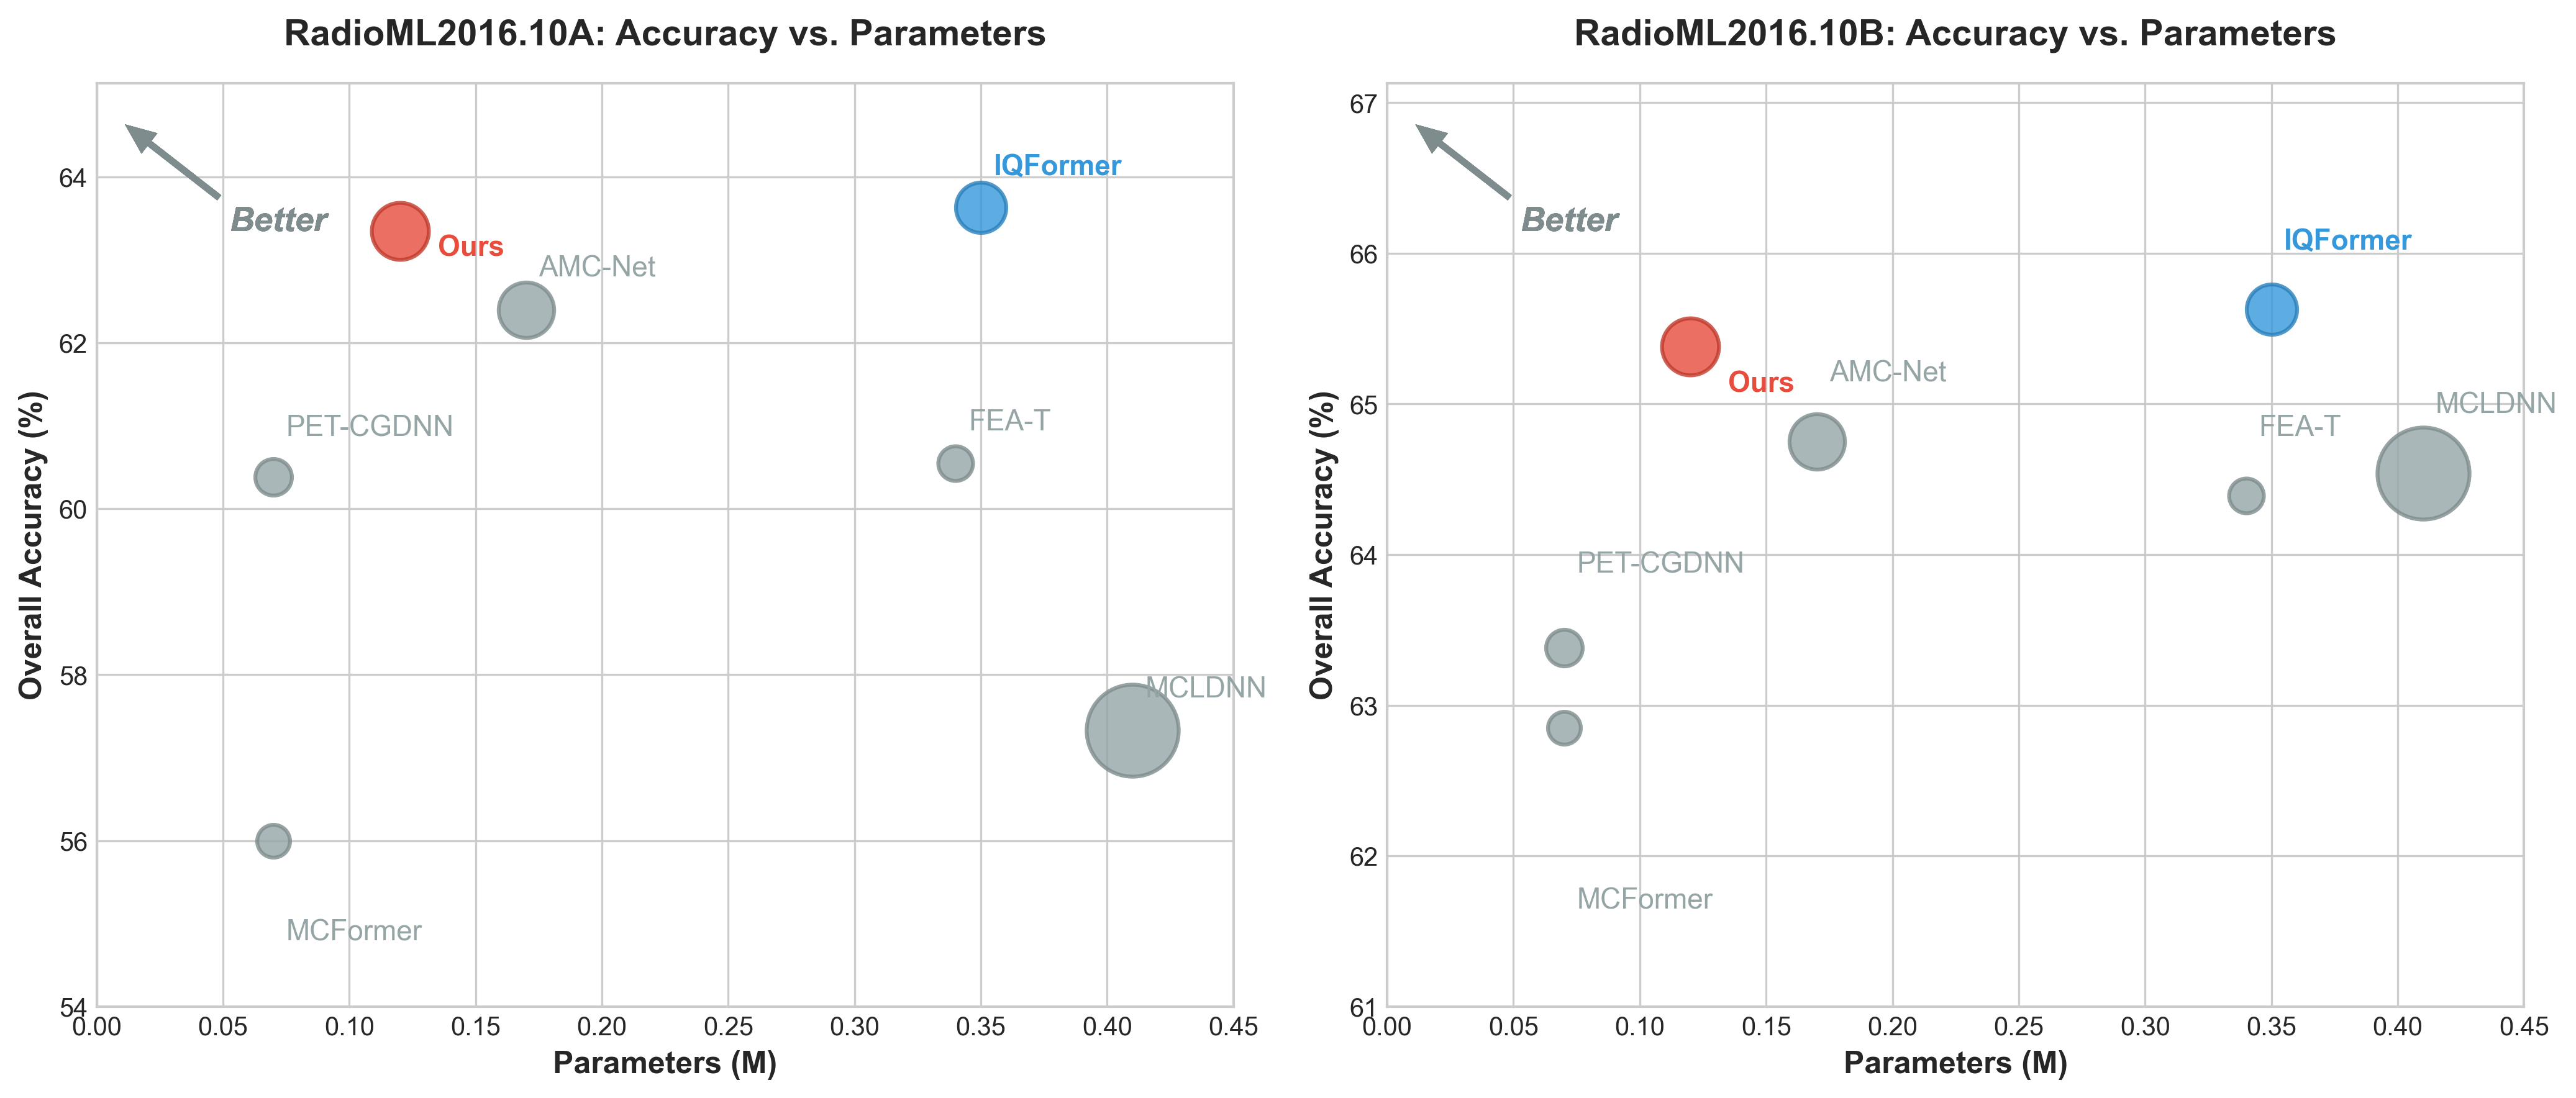
\includegraphics[width=0.9\textwidth]{Figures/param_vs_acc_bubble.png}}
		\caption{Performance trade-off comparison on RadioML2016.10A (left) and RadioML2016.10B (right). In these plots, the top-left region represents a better overall performance trade-off (i.e., fewer parameters and higher accuracy). Our proposed IQFormerLite locates at the ideal Pareto front, achieving highly competitive accuracy while significantly reducing the parameter count and computational cost compared to the baseline IQFormer and other lightweight models.}
		\label{fig:teaser_bubble}
	\end{figure}
	
	Automatic Modulation Recognition (AMR) is a key capability in modern wireless systems and supports applications such as cognitive radio, software-defined radio, spectrum sensing, and non-cooperative communications \cite{xu2020spatiotemporalmultichannela}.
	By inferring the modulation format from a received signal without prior knowledge, AMR enables adaptive receivers to operate efficiently in complex and time-varying electromagnetic environments.
	
	Classical approaches, including likelihood-based methods \cite{zhu2018likelihoodbasedalgorithm, dulek2017Onlinehybrid} and feature-based pipelines \cite{huang2017Automaticmodulation, ma2019Automaticmodulation}, established the foundations of this field.
	In practice, however, these methods often depend on accurate channel priors and hand-crafted features, which can reduce robustness under multipath fading and impulsive noise.
	
	Deep learning has made AMR more robust by supporting end-to-end recognition from raw or lightly processed inputs.
	Convolutional Neural Networks (CNNs) are widely used to learn discriminative patterns from raw I/Q sequences or signal-derived representations \cite{oshea2016Convolutionalradiob, oshea2018Overtheairdeepa, wang2019Datadrivendeepa}, while Recurrent Neural Networks (RNNs), especially Long Short-Term Memory (LSTM) networks, capture temporal structure in sequential signals \cite{chen2020Automaticmodulation, liu2021Automaticmodulation, ke2022Realtimeradioa}.
	Hybrid CNN--LSTM models combine spatial and temporal cues and can improve recognition accuracy \cite{njoku2021CGDNetEfficientb, wang2021MultidimensionalCNNLSTM, zhang2020Automaticmodulation}.
	Transformer-based designs have also been explored to model global correlations beyond the local receptive field of CNNs \cite{rashvand2024Enhancingautomatic, hou2024ClSTconvolutional, zhang2024CTRNetautomatica}.
	In parallel, several works map signals to image-like representations, including STFT spectrograms and constellation graphs \cite{chen2022SigNetnovel, lin2022Modulationrecognition, ghasemzadeh2023GGCNNefficiencymaximizing}.
	
	Despite the performance gains of these architectures, improved recognition accuracy often comes at the cost of substantial model complexity and computational redundancy. Wireless systems typically operate under tight resource constraints, relying on battery power or energy harvesting while requiring real-time processing. Consequently, deploying high-capacity models on edge devices is often impractical due to excessive memory and power demands \cite{baishya2024Edgeefficientdeep}. While lightweight AMR designs like IQFormer \cite{shao2025IQFormernovel} have improved the balance between complexity and accuracy, a gap remains between theoretical efficiency and actual hardware performance.
	
	Specifically, low theoretical complexity does not always ensure fast execution on physical hardware. Many pipelines, including IQFormer, rely on serial components like LSTMs that limit parallelism on Neural Processing Units (NPUs). Although self-attention mechanisms enable global context modeling \cite{vaswani2017Attentionall}, their quadratic computational cost is often too high for real-time embedded applications. Furthermore, frequency-domain feature extraction typically relies on fixed-basis transforms such as the STFT \cite{lin2022Learningtimefrequencya}, which increases memory traffic and does not adapt to non-stationary signals. Developing models that balance recognition accuracy with efficient hardware deployment therefore remains an open challenge.
	
	This paper introduces IQFormerLite, a hardware-efficient framework for AMR optimized for the Rockchip RK3588 NPU. As visually summarized in Figure \ref{fig:teaser_bubble}, our framework achieves an optimal Pareto trade-off, maintaining highly competitive accuracy while significantly compressing the model size compared to existing baselines. The architecture replaces sequential components and attention-based token mixing with a large-kernel convolutional design. Following Partial Large Kernel (PeLK) theory \cite{chen2024PeLKParameterefficient}, which suggests that large-kernel convolutions can achieve an effective receptive field (ERF) comparable to Transformers, IQFormerLite uses a Large-Kernel Global Context (LKGC) module instead of Efficient Additive Attention (EAA) \cite{shaker2023SwiftFormerEfficient}. This approach removes the serial bottlenecks inherent in recurrent structures and produces an operator graph better suited to NPU compilers. Additionally, IQFormerLite addresses the constraints of fixed spectral transforms using a Learnable KAN-based Filterbank (LKF). Drawing on the Kolmogorov--Arnold representation theorem \cite{kolmogorov1961representationcontinuous, liu2025KANKolmogorovarnoldc}, the LKF replaces static linear weights with learnable univariate non-linear functions via a FastKAN formulation \cite{li2024Kolmogorovarnoldnetworks}. This design treats spectral analysis as optimized 1D non-linear convolutions, allowing frequency-aware features to be extracted from raw I/Q sequences with minimal parameter growth.
	
	The main contributions of this work are as follows:
	\begin{itemize} 
		\item Hardware-Aware Architecture: We propose IQFormerLite, a streamlined architecture optimized for edge NPUs. By replacing serial LSTMs and attention mechanisms with a parallel-friendly LKGC module, we reduce serialization bottlenecks and parameter overhead while maintaining a broad effective receptive field. 
		\item Adaptive Spectral Feature Extraction: We introduce the Learnable KAN-based Filterbank (LKF). Unlike rigid STFT or linear convolutions, the LKF uses the non-linear approximation capabilities of Kolmogorov--Arnold Networks (KAN) to adaptively extract frequency-domain features, improving the representation of complex and non-stationary modulations. 
		\item Edge-Ready Validation: We provide a deployment benchmark on the Rockchip RK3588 NPU. demonstrating that IQFormerLite optimizes the trade-off between recognition accuracy and inference latency. In doing so, we bridge the gap between theoretical architecture design and the practical demands of industrial-grade real-time inference.
	\end{itemize}
	
	
	\section{Related Works}
	This section reviews the literature on Automatic Modulation Recognition (AMR), specifically focusing on model compression and efficient deployment. We first discuss developments in lightweight architecture design and then examine knowledge distillation and pruning strategies tailored for resource-constrained environments.
	
	\subsection{Lightweight Structure Design}
	Lightweight AMR for edge NPUs has shifted focus from reducing parameter counts to utilizing hardware-deployable operator sets, as end-to-end latency is often driven by kernel availability and memory traffic rather than FLOPs alone. Consequently, recent studies favor CNN-based backbones built on dense, accelerator-friendly primitives, such as depthwise and separable convolutions. These designs typically avoid operators that perform poorly on NPUs, including attention blocks, recurrent units like LSTMs, and STFT-based front-ends. For instance, CDSCNN employs complex-valued depthwise separable convolutions to lower computational costs while maintaining I/Q modeling performance \cite{xiao2023Complexvalueddepthwisea}. SCNN uses separable convolutions as a primary building block to balance accuracy and complexity \cite{fu2022Lightweightautomatic}, while ULCNN integrates complex-valued kernels with channel-mixing operations to match the performance of larger baselines with fewer parameters \cite{guo2024Ultralightconvolutional}. Beyond manual design, architecture search has been used to automatically identify efficient operators under strict resource budgets \cite{zhang2023Lightweightautomatic}. Recent analyses further suggest that many high-performing models remain over-parameterized for edge devices, highlighting the need for operator factorization and compression-friendly backbones \cite{baishya2024Edgeefficientdeep}.
	
	
	\subsection{Knowledge Distillation}
	Knowledge Distillation (KD) trains a compact model to match the behavior of a larger model and can improve the accuracy of lightweight architectures \cite{lin2024Glrseigreen}.
	Large models often provide strong performance but incur high computational and memory costs, while small models are efficient but may underfit.
	KD reduces this gap by transferring the function mapping of a teacher network to a student network.
	Qi et al.\ \cite{qi2023FedBKDHeterogenous} proposed a bidirectional KD framework for federated learning that improves performance while preserving privacy.
	Chen et al.\ \cite{chen2024Learndefend} applied KD to transfer both recognition and adversarial defense knowledge from a teacher model to a student model, improving robustness and accuracy under a reduced budget.
	
	\subsection{Pruning}
	Pruning removes low-importance weights or channels to reduce resource usage and accelerate inference \cite{molchanov2017Pruningconvolutional}.
	Deep learning models often contain redundant parameters, and sparsification can reduce compute with limited accuracy loss.
	Lin et al.\ \cite{lin2020Improvedneural} pruned convolutional filters in VT-CNN2 by identifying inactive or weakly activated filters and reported reduced overfitting under higher pruning rates.
	Chen et al.\ \cite{chen2024Channelpruning} estimated channel importance by coupling convolution and Batch Normalization (BN) statistics and applied structured pruning to remove unimportant filters.
	In practice, a compact backbone remains central: lightweight design provides the base, pruning removes redundancy, and KD transfers predictive behavior to improve accuracy under tight constraints.
	
	\section{Methodology}
	
	\subsection{Overview of the IQFormerLite Framework}
	
	\begin{figure}[htbp]
		\begin{adjustwidth}{-\extralength}{0cm}
			\centering
			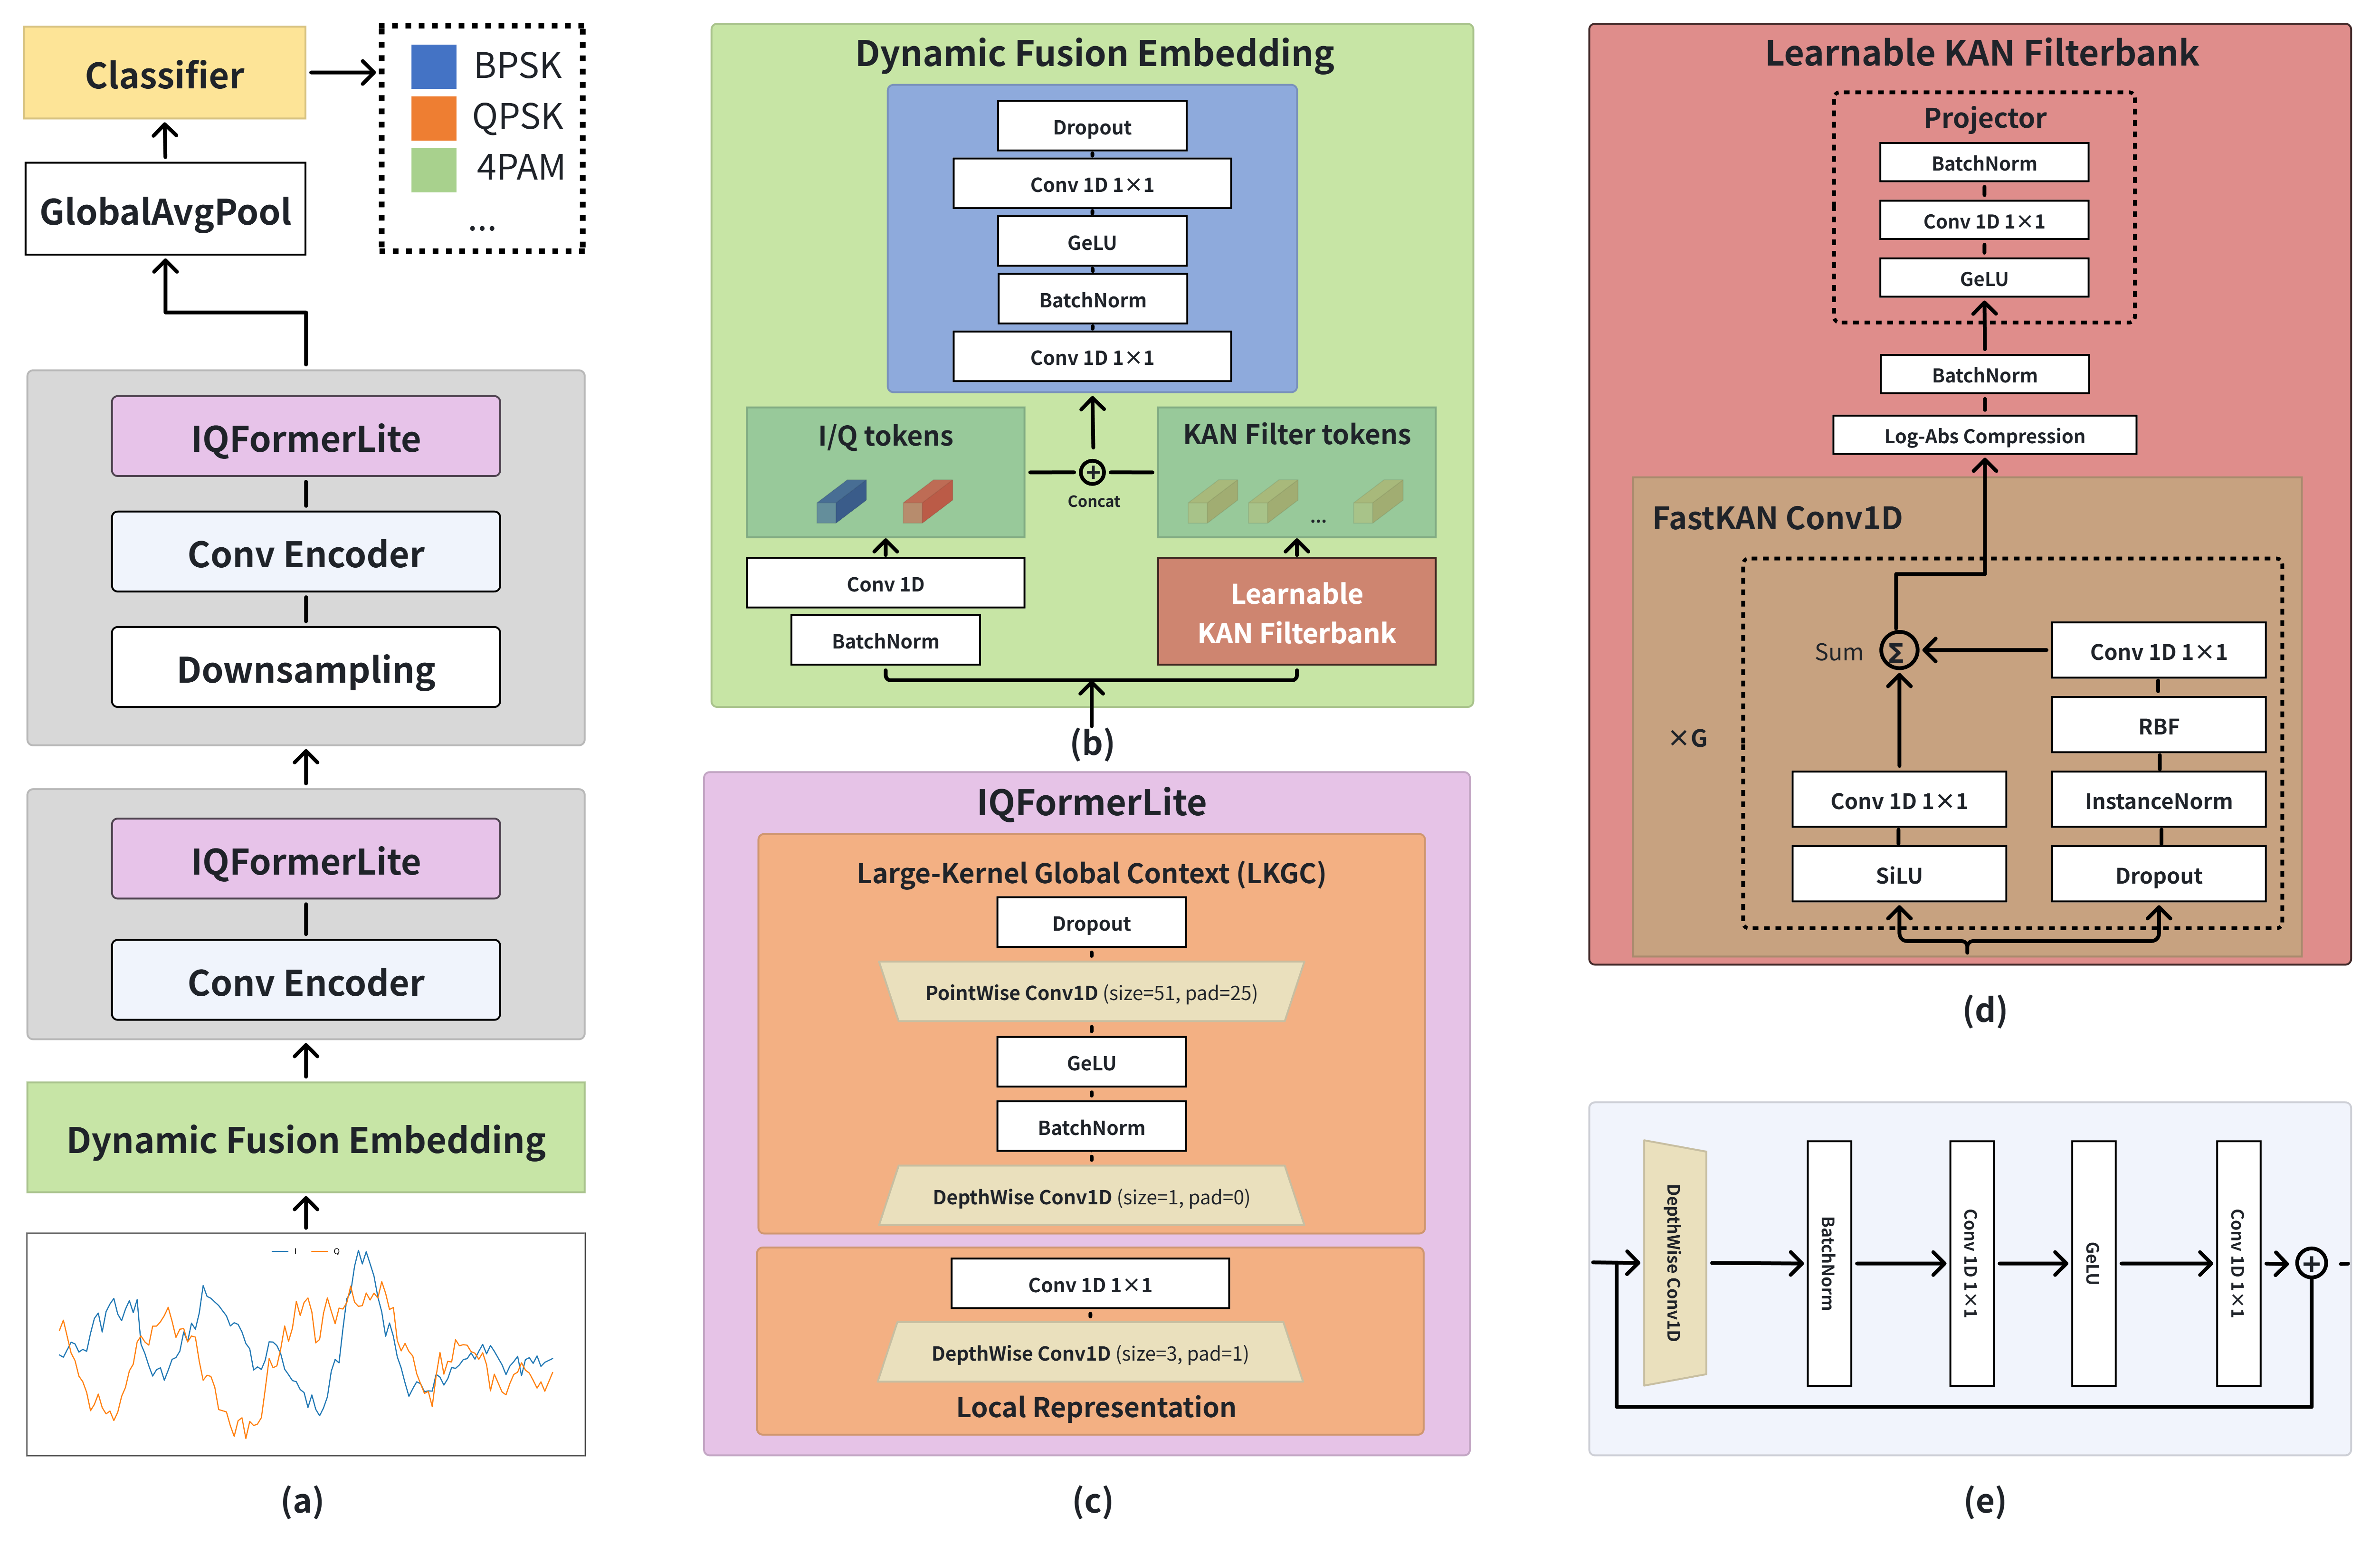
\includegraphics[width=0.9\linewidth]{Figures/overview.png}
		\end{adjustwidth}
		\caption{The overall architecture of IQFormerLite. (a) The hierarchical pipeline processing raw I/Q signals. (b) The Dynamic Fusion Embedding module integrating the Learnable KAN Filterbank. (c) The IQFormerLite Encoder Block featuring the Large-Kernel Global Context (LKGC) mechanism. (d) The internal structure of the Learnable KAN Filterbank. (e) The Conv Encoder Block for local feature refinement.}
		\label{fig:overview}
	\end{figure}
	
	The IQFormerLite framework builds on the hierarchical design of IQFormer \cite{shao2025IQFormernovel} and is tailored to resource-constrained edge NPUs.
	As shown in Fig.~\ref{fig:overview}, the multi-stage structure of the baseline is retained, but two hardware-driven changes are introduced.
	A Dynamic Fusion Embedding module incorporates a Learnable KAN-based Filterbank (LKF) to capture frequency-domain features directly from raw I/Q inputs.
	The backbone replaces attention with Large-Kernel Global Context (LKGC) blocks, which model long-range dependencies using a convolutional operator graph.
	The resulting semantic features are passed to a lightweight classifier for modulation prediction.
	This design avoids matrix-heavy and serial operators used in the original IQFormer and better matches the parallel execution model of edge hardware such as Rockchip RK3588.
	It also fits the constraints of common edge compiler stacks (for example, RKNN-Toolkit), which benefit from operator fusion and static graph execution for efficient deployment.
	
	\subsection{Large-Kernel Global Context (LKGC) Block}
	\label{sec:lkgc}
	
	In many AMR architectures, attention is used to model long-range dependencies in signal sequences.
	On edge devices, however, theoretical complexity reductions do not always translate into hardware efficiency.
	Even linear attention variants such as Efficient Additive Attention (EAA) \cite{shaker2023SwiftFormerEfficient} often require fragmented operations, including dynamic matrix multiplications, global reductions, and broadcasting.
	These patterns can lead to irregular memory access and reduce the benefit of on-chip buffering, which increases latency on NPUs.
	IQFormerLite instead follows the large-kernel design direction from computer vision \cite{chen2024PeLKParameterefficient}, where expansive convolutions approximate the global Effective Receptive Field (ERF) of Transformer-style models.
	Accordingly, the EAA module is replaced with a Large-Kernel Global Context (LKGC) block that expresses context modeling as a fully convolutional operator graph.
	
	Global context aggregation uses a large-kernel depthwise convolution with $K{=}51$ to collect temporal information over a wide window on a per-channel basis.
	Unlike attention, this operation follows a contiguous sliding-window access pattern, which supports efficient prefetching and reduces off-chip memory traffic.
	For an input feature map $\mathbf{X}$, the intermediate feature $\mathbf{Y}_{dw}$ is computed as
	\begin{equation}
		\mathbf{Y}_{dw} = \mathbf{W}_{dw} \ast \mathbf{X},
	\end{equation}
	where $\mathbf{W}_{dw}$ is a depthwise kernel of size $K$, with padding $P = \lfloor K/2 \rfloor$ to preserve the sequence length and groups equal to the channel dimension $C$.
	
	Channel mixing then applies Batch Normalization (BN) and GELU activation, followed by a pointwise convolution to exchange information across channels.
	The output $\mathbf{Y}_{out}$ is
	\begin{equation}
		\mathbf{Y}_{out} = \mathbf{W}_{pw} \cdot \sigma(\text{BN}(\mathbf{Y}_{dw})),
	\end{equation}
	where $\mathbf{W}_{pw}$ denotes the pointwise convolution weights and $\sigma$ denotes GELU.
	This design removes query--key--value projections and softmax-style operators and yields a graph composed of common convolutional primitives.
	Such Conv--BN--Act patterns are typically well supported by NPU compilers, enabling operator fusion and improving real-time performance.
	
	\subsection{Learnable KAN-based Filterbank (LKF)}
	\label{sec:lkf}
	
	Fixed-basis transforms such as STFT can be costly and may not capture non-stationary spectral patterns efficiently.
	IQFormerLite therefore uses a Learnable KAN-based Filterbank (LKF) that represents each convolution kernel as a learnable non-linear function under the FastKAN framework \cite{li2024Kolmogorovarnoldnetworks, drokin2024Kolmogorovarnoldconvolutions}.
	This parameterization keeps the computation compatible with edge NPUs while increasing flexibility beyond static scalar weights.
	
	The FastKAN formulation decomposes the operation into a linear approximation path and a non-linear residual path.
	For an input signal $\mathbf{X}$, the $m$-th filter is
	\begin{equation}
		\Phi_m(\mathbf{X}) = \underbrace{\mathbf{W}_{base} * \sigma(\mathbf{X})}_{\text{Global Linear}} + \underbrace{\mathbf{W}_{spline} * \Psi(\mathbf{\hat{X}})}_{\text{Local Non-Linear}},
	\end{equation}
	where $*$ denotes convolution with temporal kernel size $K$, $\sigma$ is the SiLU activation, and $\mathbf{W}_{base}$ models global linear structure.
	
	The non-linearity $\Psi(\cdot)$ is implemented with Radial Basis Functions (RBFs) over a learnable grid.
	Let $G$ be the grid size (the number of RBF centers).
	For a normalized scalar input $x$, the $g$-th basis function is
	\begin{equation}
		\Psi_g(x) = \exp\left( -\left( \frac{x - \mu_g}{h} \right)^2 \right), \quad g=1,\dots,G,
		\label{eq:rbf}
	\end{equation}
	where $\mu_g$ denotes grid centers initialized uniformly over a bounded range $[-R, R]$ (the grid range), and $h$ is a smoothing factor determined by the grid granularity.
	This expansion supports non-monotonic frequency responses within receptive field $K$ and remains vectorized as element-wise tensor operations.
	
	After KAN convolution, a log-abs transformation compresses the dynamic range of the learned spectral features:
	\begin{equation}
		\mathbf{Y}_{spec} = \log(1 + |\Phi(\mathbf{X})| + \epsilon).
	\end{equation}
	This step emphasizes transient patterns and stabilizes the feature scale before fusion.
	
	\section{Experiments and Results}
	\label{sec:ExpRes}
	
	\subsection{Evaluation Datasets}
	We evaluate on two benchmark datasets from the RadioML series, RadioML2016.10A and RadioML2016.10B \cite{oshea2016Convolutionalradiob}.
	Both datasets cover SNRs from $-20$~dB to $+18$~dB.
	Dataset statistics are summarized in Table~\ref{tab:datasets}.
	
	\begin{table}[htbp]
		\centering
		\caption{Summary of RadioML Datasets}
		\label{tab:datasets}
		\renewcommand{\arraystretch}{1.2}
		\begin{tabular}{lcccc}
			\toprule[1.5pt]
			\textbf{Dataset} & \textbf{\#Samples} & \textbf{Input Shape} & \textbf{Classes} & \textbf{SNR Range (dB)} \\
			\midrule
			RML2016.10A & 220,000   & $2 \times 128$ & 11 & $-20 \sim 18$ (Step 2) \\
			RML2016.10B & 1,200,000 & $2 \times 128$ & 10 & $-20 \sim 18$ (Step 2) \\
			\bottomrule[1.5pt]
		\end{tabular}
	\end{table}
	
	\subsection{Implementation Details}
	The experiments follow a common workflow with offline training on a server and on-device inference on the target edge platform.
	
	All models are trained in PyTorch on a server equipped with an NVIDIA A800 80GB GPU.
	AdamW is used with batch size 1{,}024 and an initial learning rate of $1 \times 10^{-3}$.
	A \texttt{ReduceLROnPlateau} scheduler reduces the learning rate by a factor of 0.5 with patience of 3 epochs.
	Early stopping uses patience of 10 epochs with a maximum of 60 epochs.
	Cross-entropy loss is used for optimization.
	
	Deployment evaluation uses Orange Pi 5 Plus (Fig.~\ref{fig:orangepi5}) as the edge platform.
	The device integrates Rockchip RK3588 with an octa-core CPU (4$\times$Cortex-A76 @ 2.4GHz + 4$\times$Cortex-A55 @ 1.8GHz) and an NPU providing 6~TOPS of INT8 compute.
	The system runs Orange Pi OS 1.2.0 (Jammy), based on Ubuntu 22.04~LTS, with vendor kernel 6.1.43 (aarch64).
	To reduce benchmarking variance, the device runs in performance mode with fan cooling enabled to avoid thermal throttling.
	
	\begin{figure}[htbp]
		\centering
		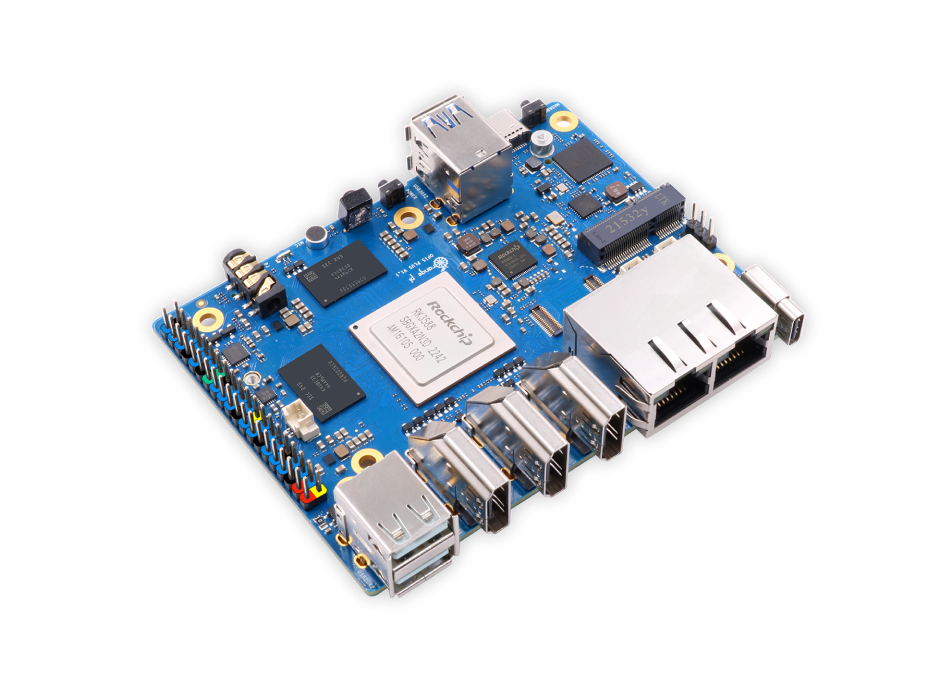
\includegraphics[width=0.5\linewidth]{Figures/orangepi5.png}
		\caption{The experimental hardware platform. The Orange Pi 5 Plus is equipped with the Rockchip RK3588 SoC, which integrates the tri-core NPU providing 6 TOPS of computing power.}
		\label{fig:orangepi5}
	\end{figure}
	
	To bridge offline training and on-device execution, we adopt a PyTorch $\to$ ONNX $\to$ RKNN conversion pipeline.
	Trained FP32 PyTorch models are exported to ONNX with a fixed input shape and then simplified with onnx-sim to remove redundant operators and fold constants, yielding a compiler-friendly graph.
	We compile the optimized ONNX model with RKNN-Toolkit2 and apply post-training quantization (PTQ) to target INT8 execution.
	Quantization parameters are estimated using a calibration set of 500 samples drawn from the validation split.
	The resulting \texttt{.rknn} models are executed on RK3588 via the RKNN Python Runtime API for accuracy validation and performance profiling.
	
	\subsection{Comparisons With SOTA Deep Models}
	This section compares IQFormerLite with representative deep models, including IQFormer \cite{shao2025IQFormernovel}, MCLDNN \cite{xu2020spatiotemporalmultichannelc}, MCFormer \cite{hamidi-rad2021MCformertransformera}, PET-CGDNN \cite{zhang2021efficientdeepa}, AMC-Net \cite{zhang2023AMCneteffective}, and FEA-T \cite{chen2023Abandonlocality}.
	The evaluation considers both recognition accuracy and computational efficiency to quantify practical benefits under edge constraints.
	
	As summarized in Table~\ref{tab:sota_compare}, IQFormer reaches an overall accuracy of $63.60 \pm 0.11\%$ on RadioML2016.10A and $65.42 \pm 0.18\%$ on RadioML2016.10B. IQFormerLite remains highly competitive, maintaining accuracies of $63.18 \pm 0.22\%$ and $65.51 \pm 0.13\%$, respectively. This comparable performance, with a small gap on RadioML2016.10A and a slight advantage on RadioML2016.10B, is paired with a substantial gain in efficiency: IQFormerLite utilizes only $0.12$~M parameters compared to the $0.35$~M of IQFormer, representing a $65.7\%$ reduction in model size. Compared to existing lightweight architectures, IQFormerLite consistently outperforms AMC-Net ($0.17$~M parameters) and delivers a significant accuracy improvement over MCFormer, with gains of $7.89$ percentage points on RadioML2016.10A and $2.29$ percentage points on RadioML2016.10B. These results demonstrate that IQFormerLite effectively balances the trade-off between recognition performance and resource constraints.

	
	\begin{table}[htbp]
		\caption{Comparison of model complexity and accuracy on two datasets (A: RadioML2016.10A, B: RadioML2016.10B). Accuracy values are reported as mean $\pm$ standard deviation over five random seeds. \textbf{Bold} indicates the best result, and \underline{underline} indicates the second-best result.}
		\label{tab:sota_compare}
		\renewcommand{\arraystretch}{1.25}
		\centering
		\small
		\setlength{\tabcolsep}{3pt}
		
		\newcolumntype{Y}{>{\centering\arraybackslash}X}
		
		\begin{tabularx}{\linewidth}{@{}l c c c Y Y Y@{}}
			\toprule
			\multirow{2}{*}{\textbf{Model}} &
			\multirow{2}{*}{\textbf{Dataset}} &
			\multirow{2}{*}{\makecell{\textbf{Param.}\\\textbf{(M)}}} &
			\multirow{2}{*}{\makecell{\textbf{FLOPs}\\\textbf{(M)}}} &
			\multicolumn{2}{c}{\makecell{\textbf{Avg. Acc. over SNR}\\\textbf{(\%)}}} &
			\multirow{2}{*}{\makecell{\textbf{Overall Acc.}\\\textbf{(\%)}}} \\
			\cmidrule(lr){5-6}
			& & & & \textbf{-20--0} & \textbf{0--18} & \\
			\midrule
			
			\multirow{2}{*}{MCLDNN}    & A & \multirow{2}{*}{0.41} & \multirow{2}{*}{97.00} & $32.09 \pm 4.67$ & $78.50 \pm 8.41$ & $53.23 \pm 6.24$ \\
			& B &                       &                        & $34.84 \pm 13.89$ & $76.44 \pm 37.14$ & $53.64 \pm 24.40$ \\
			\midrule
			
			\multirow{2}{*}{MCFormer}  & A & \multirow{2}{*}{\textbf{0.07}} & \multirow{2}{*}{\textbf{5.06}} & $34.38 \pm 0.16$ & $80.47 \pm 1.85$ & $55.29 \pm 0.80$ \\
			& B &                                &                                 & $39.63 \pm 0.45$ & $91.73 \pm 0.58$ & $63.22 \pm 0.46$ \\
			\midrule
			
			\multirow{2}{*}{PET-CGDNN} & A & \multirow{2}{*}{\textbf{0.07}} & \multirow{2}{*}{8.31} & $32.82 \pm 3.47$ & $81.22 \pm 3.34$ & $54.87 \pm 3.25$ \\
			& B &                                &                        & $39.44 \pm 0.22$ & $92.34 \pm 0.09$ & $63.39 \pm 0.15$ \\
			\midrule
			
			\multirow{2}{*}{AMC-Net}   & A & \multirow{2}{*}{0.17} & \multirow{2}{*}{29.82} & $36.79 \pm 0.36$ & $87.65 \pm 0.78$ & $59.79 \pm 0.52$ \\
			& B &                       &                        & $41.38 \pm 0.12$ & $93.13 \pm 0.09$ & $64.75 \pm 0.10$ \\
			\midrule
			
			\multirow{2}{*}{FEA-T}     & A & \multirow{2}{*}{0.34} & \multirow{2}{*}{6.65} & $35.44 \pm 1.68$ & $85.82 \pm 2.26$ & $58.37 \pm 1.84$ \\
			& B &                       &                       & $34.39 \pm 13.64$ & $76.31 \pm 37.07$ & $53.35 \pm 24.23$ \\
			\midrule
			
			\multirow{2}{*}{IQFormer}  & A & \multirow{2}{*}{0.35} & \multirow{2}{*}{23.10} & $\textbf{39.50} \pm \textbf{0.30}$ & $\textbf{92.81} \pm \textbf{0.27}$ & $\textbf{63.60} \pm \textbf{0.11}$ \\
			& B &                       &                        & $\underline{42.24 \pm 0.31}$ & $\underline{93.62 \pm 0.07}$ & $\underline{65.42 \pm 0.18}$ \\
			\midrule
			
			\multirow{2}{*}{\textbf{Ours}} &
			A &
			\multirow{2}{*}{\underline{0.12}} &
			\multirow{2}{*}{32.06} &
			$\underline{39.11 \pm 0.23}$ & $\underline{92.36 \pm 0.45}$ & $\underline{63.18 \pm 0.22}$ \\
			& B & & & $\textbf{42.28} \pm \textbf{0.22}$ & $\textbf{93.75} \pm \textbf{0.05}$ & $\textbf{65.51} \pm \textbf{0.13}$ \\
			\bottomrule
		\end{tabularx}
	\end{table}

	Fig.~\ref{fig:sota_acc} complements Table~\ref{tab:sota_compare} by reporting the five-seed mean accuracy as a function of SNR.
	Both datasets follow a common pattern: accuracy is close to chance under severe noise, increases sharply in the transition region (approximately $-10$ to $0$~dB), and saturates above $0$~dB.
	Across the full SNR range, IQFormerLite remains among the strongest methods relative to the baselines.
	On RadioML2016.10A, IQFormerLite closely tracks IQFormer, with high-SNR accuracies of $92.36 \pm 0.45\%$ and $92.81 \pm 0.27\%$, respectively, indicating that most discriminative capacity is retained under compression.
	On RadioML2016.10B, IQFormerLite reaches $93.75 \pm 0.05\%$ at high SNR, compared with $93.62 \pm 0.07\%$ for IQFormer; the near overlap and narrow variation across seeds indicate comparable high-SNR performance.
	
	\begin{figure}[htbp]
		\centering
		\subfloat[\centering]{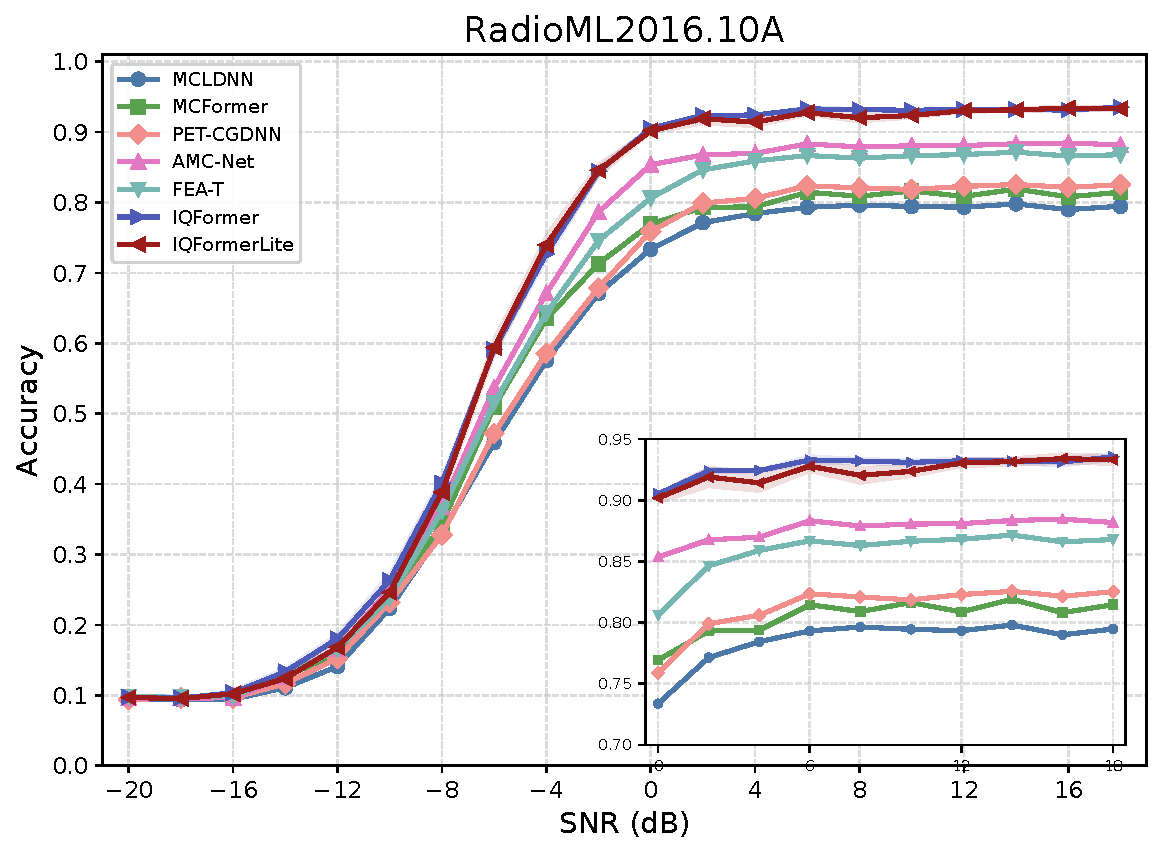
\includegraphics[width=0.49\linewidth]{Figures/RML201610a_sota_acc.pdf}\label{fig:sota_acc_a}}
		\hfill
		\subfloat[\centering]{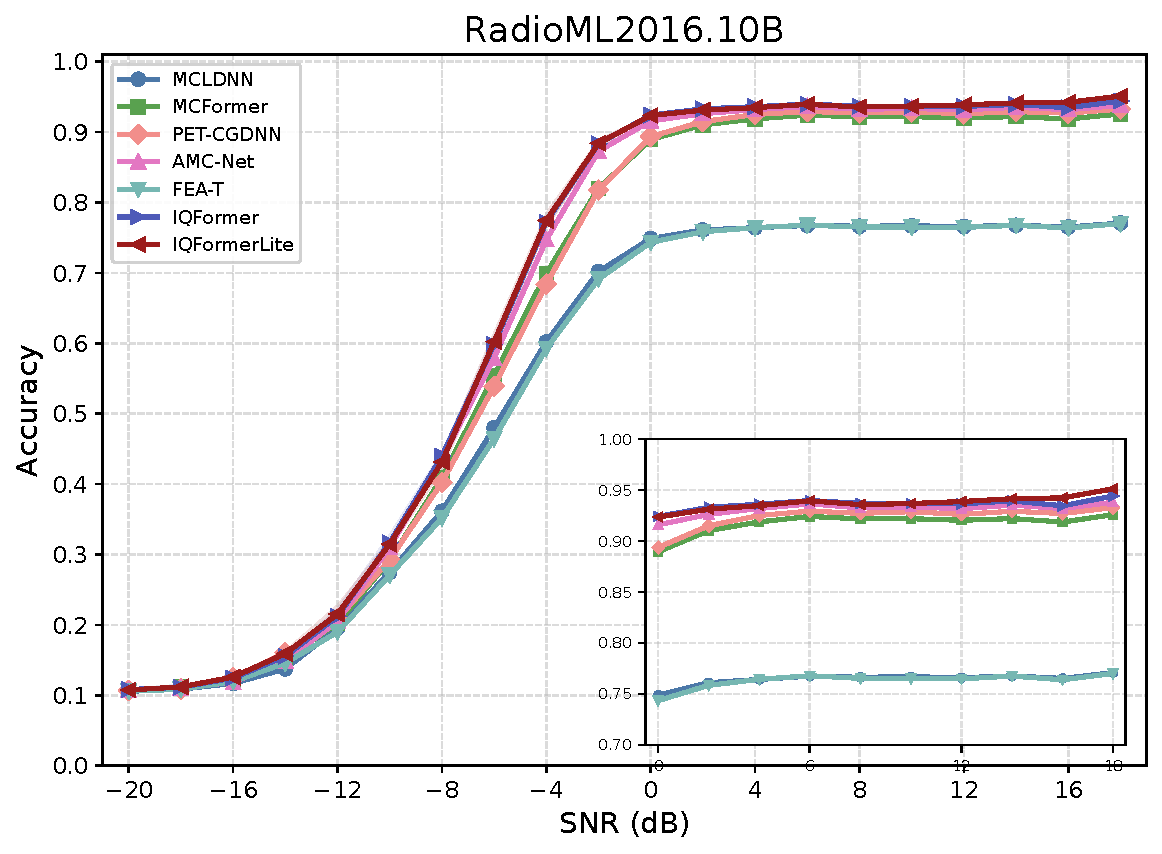
\includegraphics[width=0.49\linewidth]{Figures/RML201610b_sota_acc.pdf}\label{fig:sota_acc_b}}
		\caption{Comparison of recognition accuracy under varying SNR levels. Curves report the mean over five random seeds; shaded regions denote $\pm$ one standard deviation for IQFormer and IQFormerLite. (a) RadioML2016.10A. (b) RadioML2016.10B. \label{fig:sota_acc}}
	\end{figure}
	
	Overall, IQFormerLite improves over prior lightweight baselines while following the expected SNR-dependent trend.
	With parameters reduced from 0.35~M to 0.12~M (65.7\% compression), overall accuracy remains close to IQFormer, supporting the use of the proposed design for edge deployment.
	
	\subsection{Modulation Analysis}
	This section examines class-wise behavior to identify where compression affects recognition and how errors concentrate across modulation families.
	Fig.~\ref{fig:mod_acc_comparison}(a)--(d) reports the five-seed mean per-class accuracies of IQFormer and IQFormerLite on RadioML2016.10A and RadioML2016.10B.
	A consistent pattern appears among closely confusable analog modulations. Averaged across all evaluated SNR levels, IQFormerLite improves WBFM accuracy relative to IQFormer by $9.29$ percentage points on RadioML2016.10A and $3.00$ percentage points on RadioML2016.10B, while AM-DSB accuracy changes by $-9.10$ and $-1.54$ percentage points, respectively.
	This inverse shift suggests that compression mainly adjusts decision boundaries among overlapping classes rather than causing a uniform decline across modulation types.
	Accordingly, most behavioral changes are concentrated in a small set of ambiguous analog categories, while overall capability is largely preserved.
	
	\begin{figure}[htbp]
		\centering
		\subfloat[\centering]{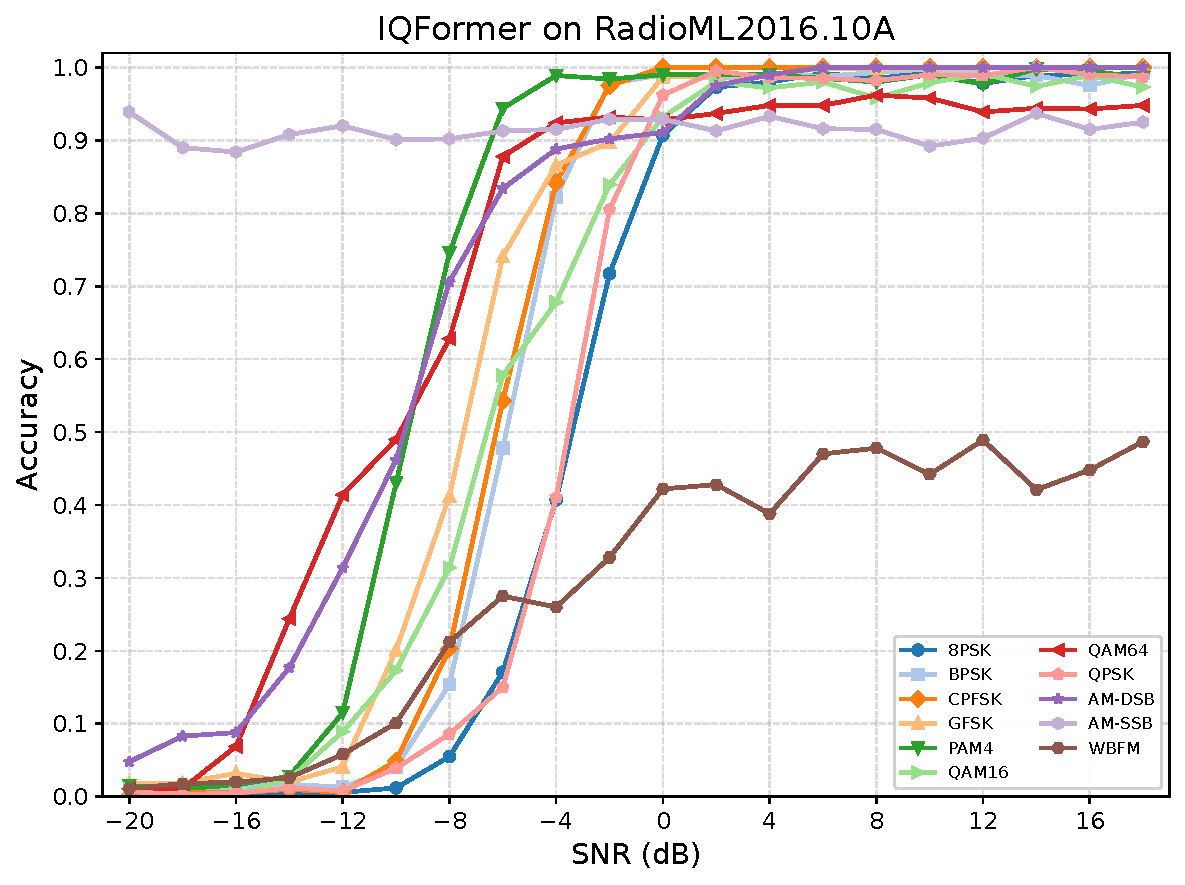
\includegraphics[width=0.49\linewidth]{Figures/RML201610a_IQFormer_mod_acc.pdf}\label{fig:mod_acc_a}}
		\hfill
		\subfloat[\centering]{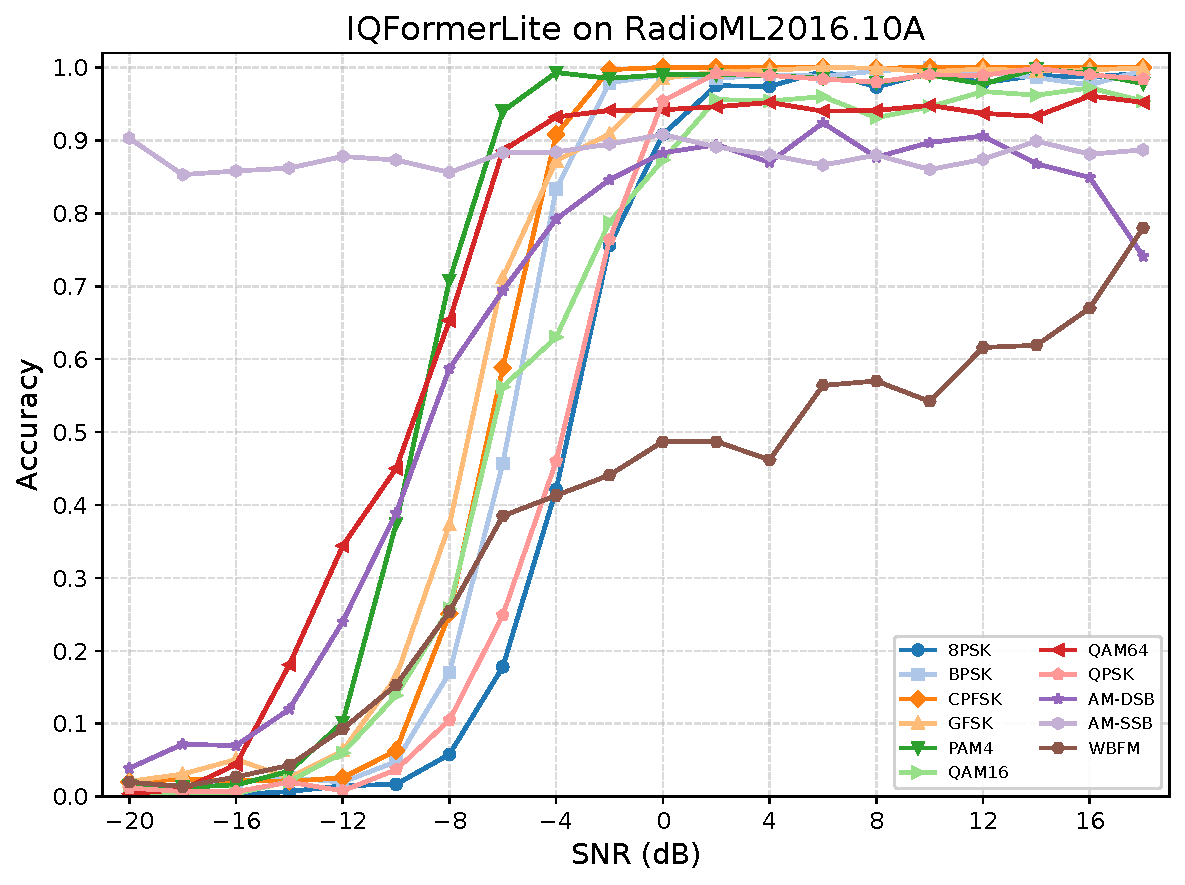
\includegraphics[width=0.49\linewidth]{Figures/RML201610a_IQFormerLite_mod_acc.pdf}\label{fig:mod_acc_b}}
		
		\vspace{6pt}
		
		\subfloat[\centering]{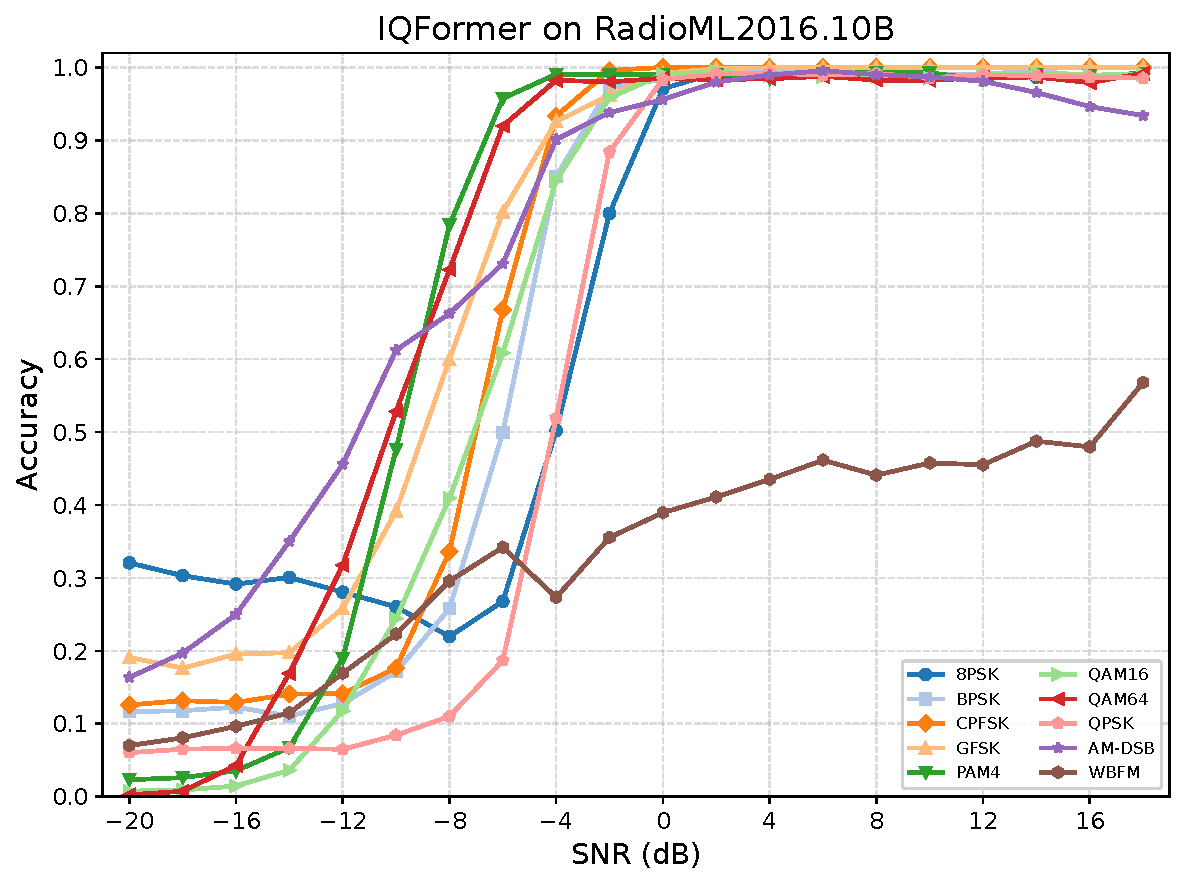
\includegraphics[width=0.49\linewidth]{Figures/RML201610b_IQFormer_mod_acc.pdf}\label{fig:mod_acc_c}}
		\hfill
		\subfloat[\centering]{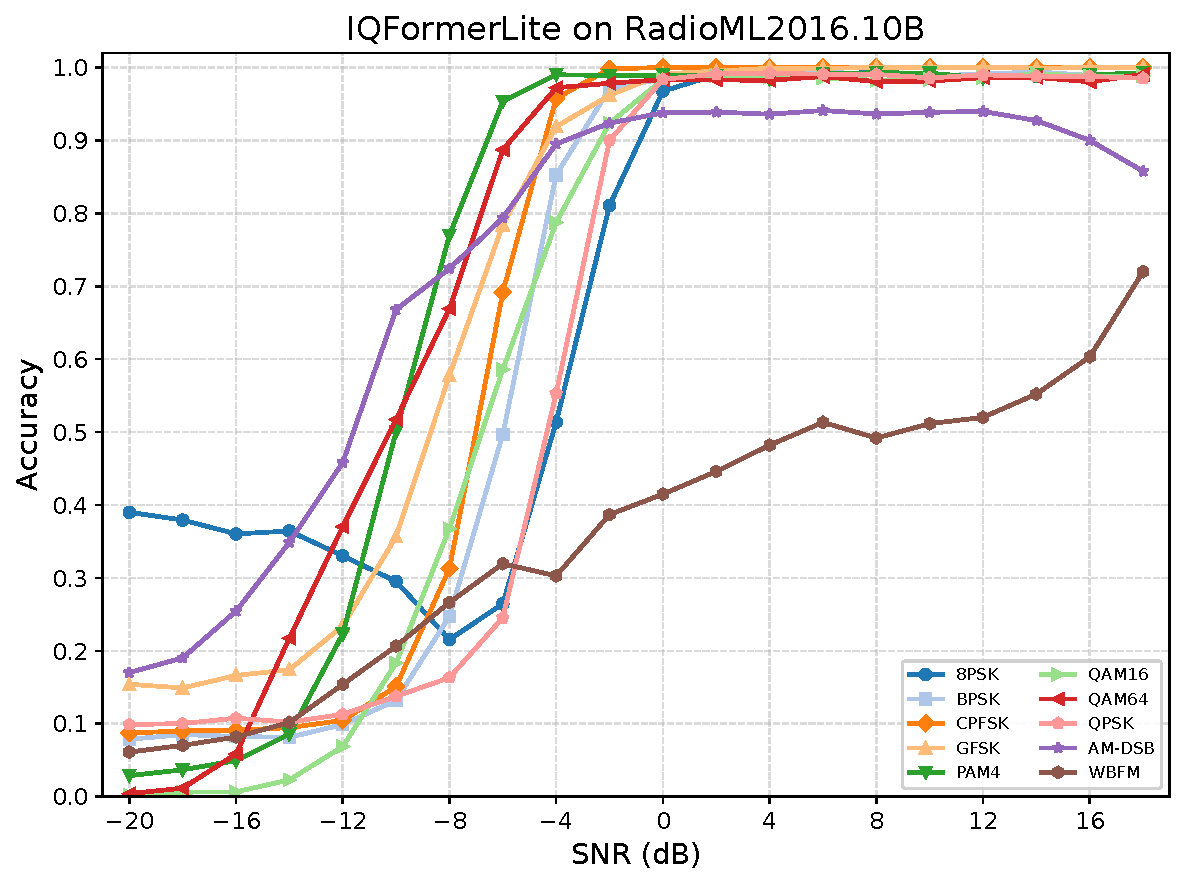
\includegraphics[width=0.49\linewidth]{Figures/RML201610b_IQFormerLite_mod_acc.pdf}\label{fig:mod_acc_d}}
		
		\caption{Comparison of per-modulation recognition accuracy between the baseline IQFormer and the proposed IQFormerLite. Curves report the mean over five random seeds.
			(a) IQFormer on RadioML2016.10A.
			(b) IQFormerLite on RadioML2016.10A.
			(c) IQFormer on RadioML2016.10B.
			(d) IQFormerLite on RadioML2016.10B.
			\label{fig:mod_acc_comparison}}
	\end{figure}
	
	To further characterize the error structure, Fig.~\ref{fig:confusion_matrix} reports confusion matrices of IQFormerLite at SNR $=-4$~dB and SNR $=2$~dB.
	Across both datasets and both SNR settings, the most prominent error mode is strong and largely unidirectional confusion from WBFM to AM-DSB.
	This confusion persists when channel conditions improve from $-4$~dB to $2$~dB, which suggests that noise alone does not explain the misrecognition.
	For example, at $2$~dB on RadioML2016.10A, 42\% of WBFM samples are predicted as AM-DSB, and the corresponding error rate increases to 58\% on RadioML2016.10B at the same SNR.
	These results are consistent with dataset-level ambiguity: segments with weak or silent analog content reduce discriminative cues and can make the I/Q statistics of WBFM resemble AM-DSB, which concentrates WBFM samples in the AM-DSB decision region.
	The same tendency remains visible under compression, aligning with the stable confusion structure observed for IQFormerLite.
	
	\begin{figure}[htbp]
		\begin{adjustwidth}{-\extralength}{0cm}
			\centering
			\subfloat[\centering RadioML2016.10A\label{fig:cm_a}]{
				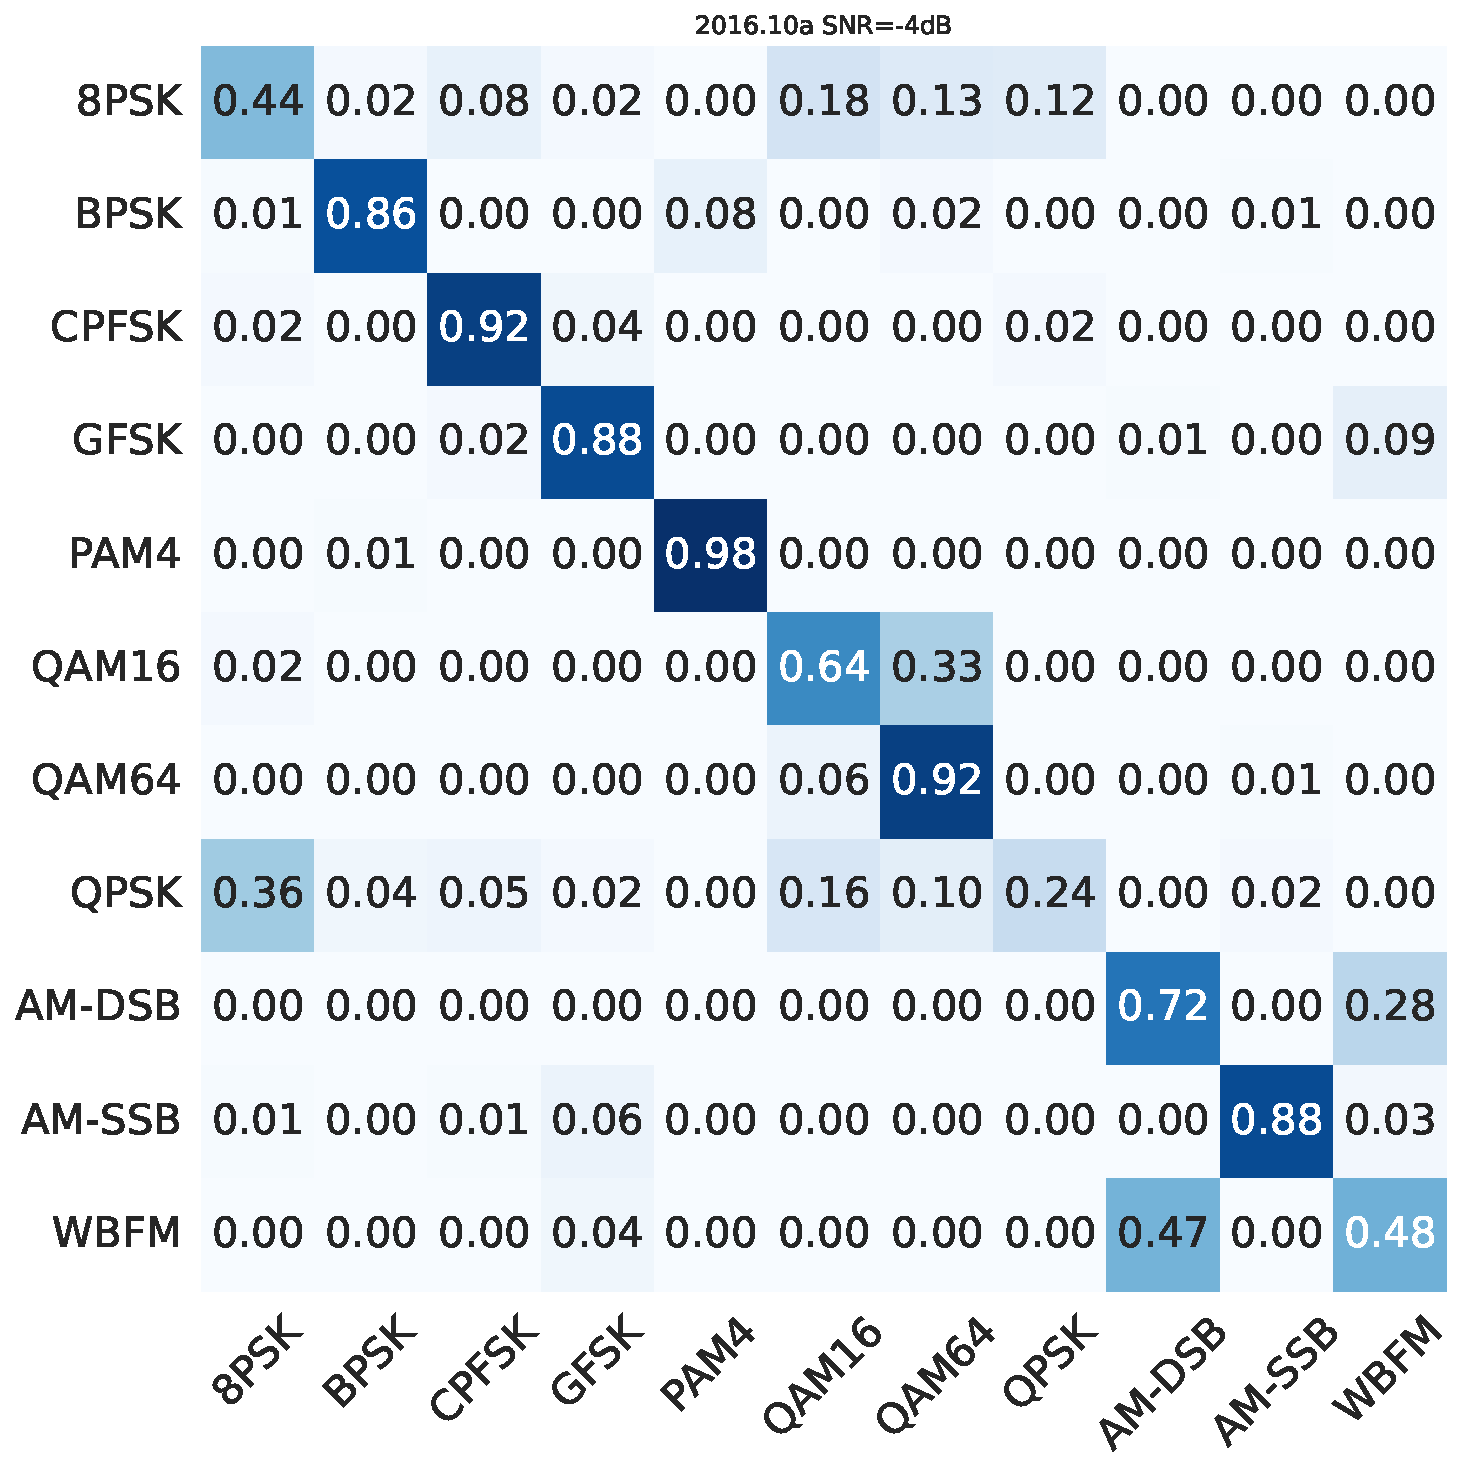
\includegraphics[width=0.24\linewidth]{Figures/IQFormerLite_RML201610A_confusionMatrix/2016.10a_-4.pdf}
				\hfill
				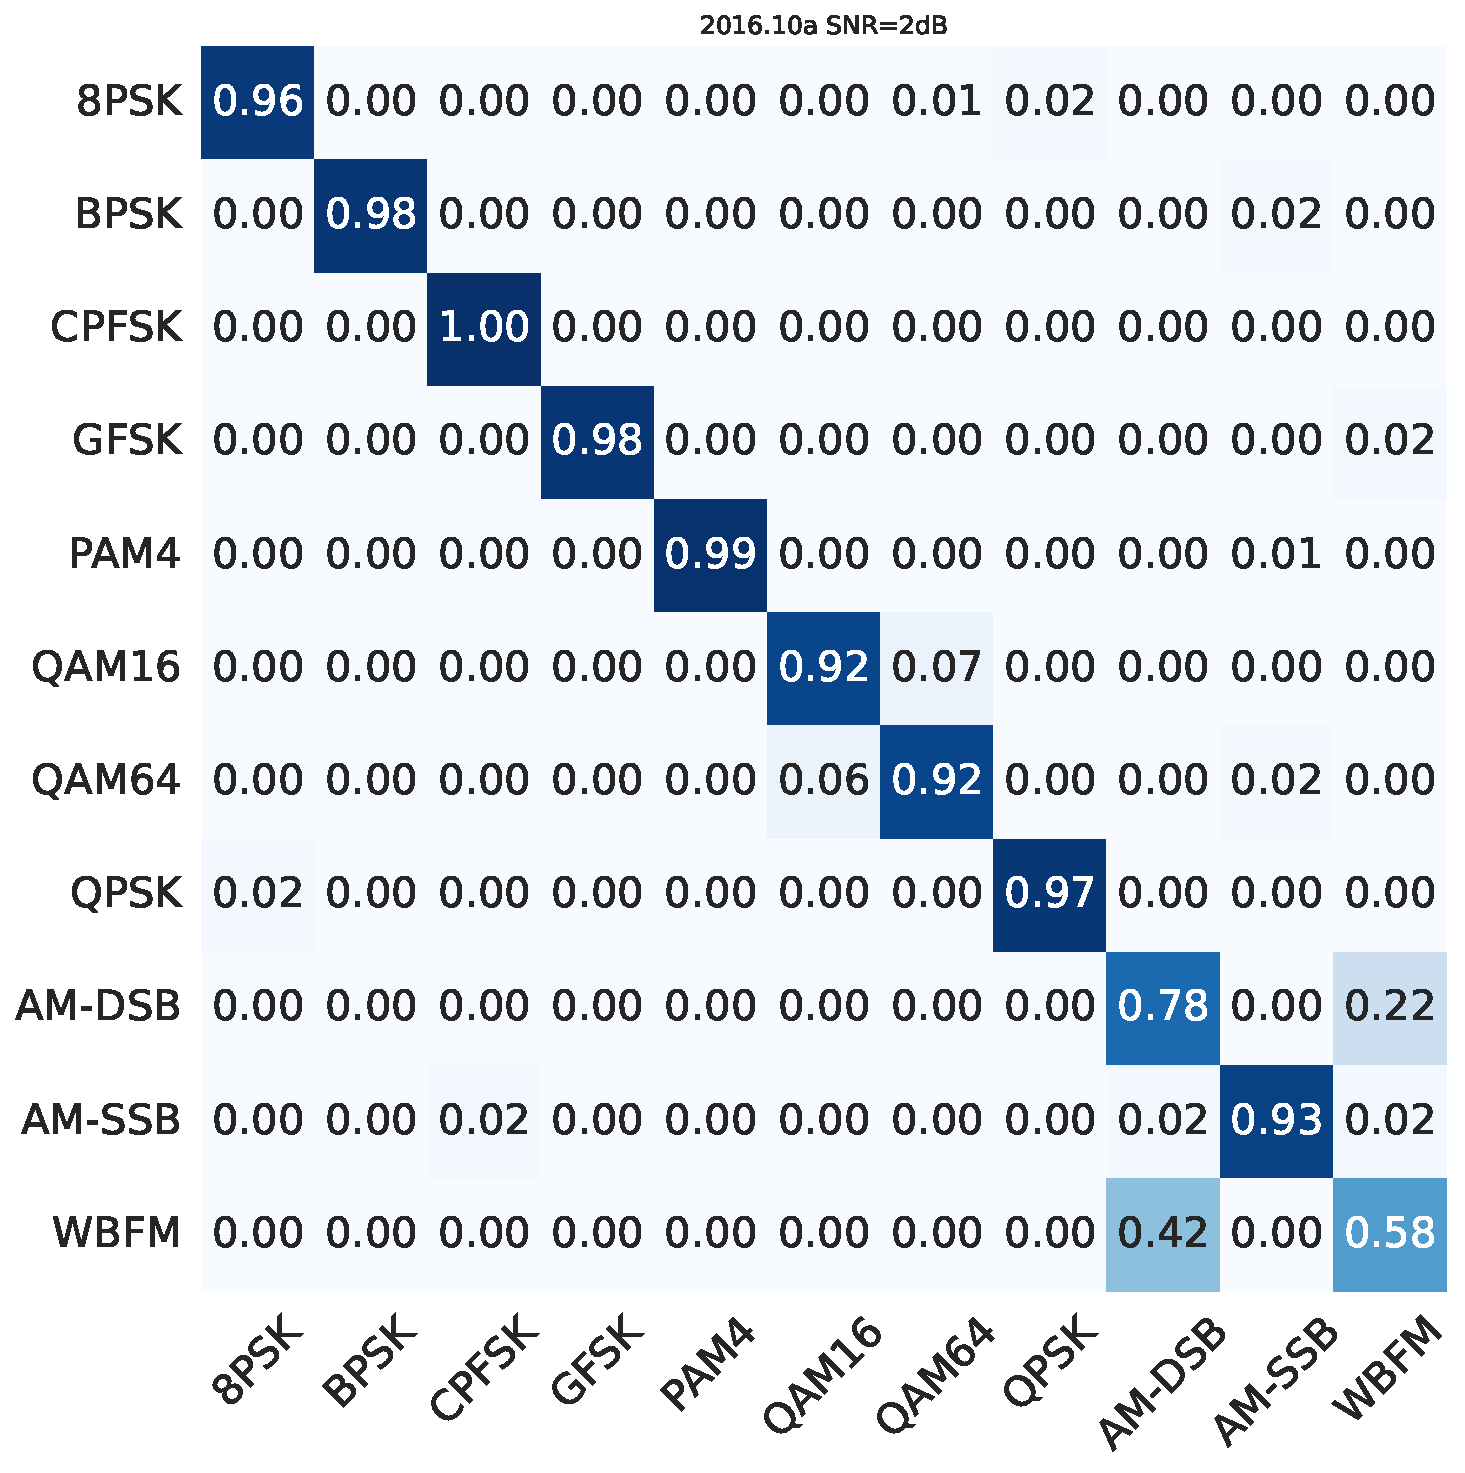
\includegraphics[width=0.24\linewidth]{Figures/IQFormerLite_RML201610A_confusionMatrix/2016.10a_2.pdf}
			}
			\hfill
			\subfloat[\centering RadioML2016.10B\label{fig:cm_b}]{
				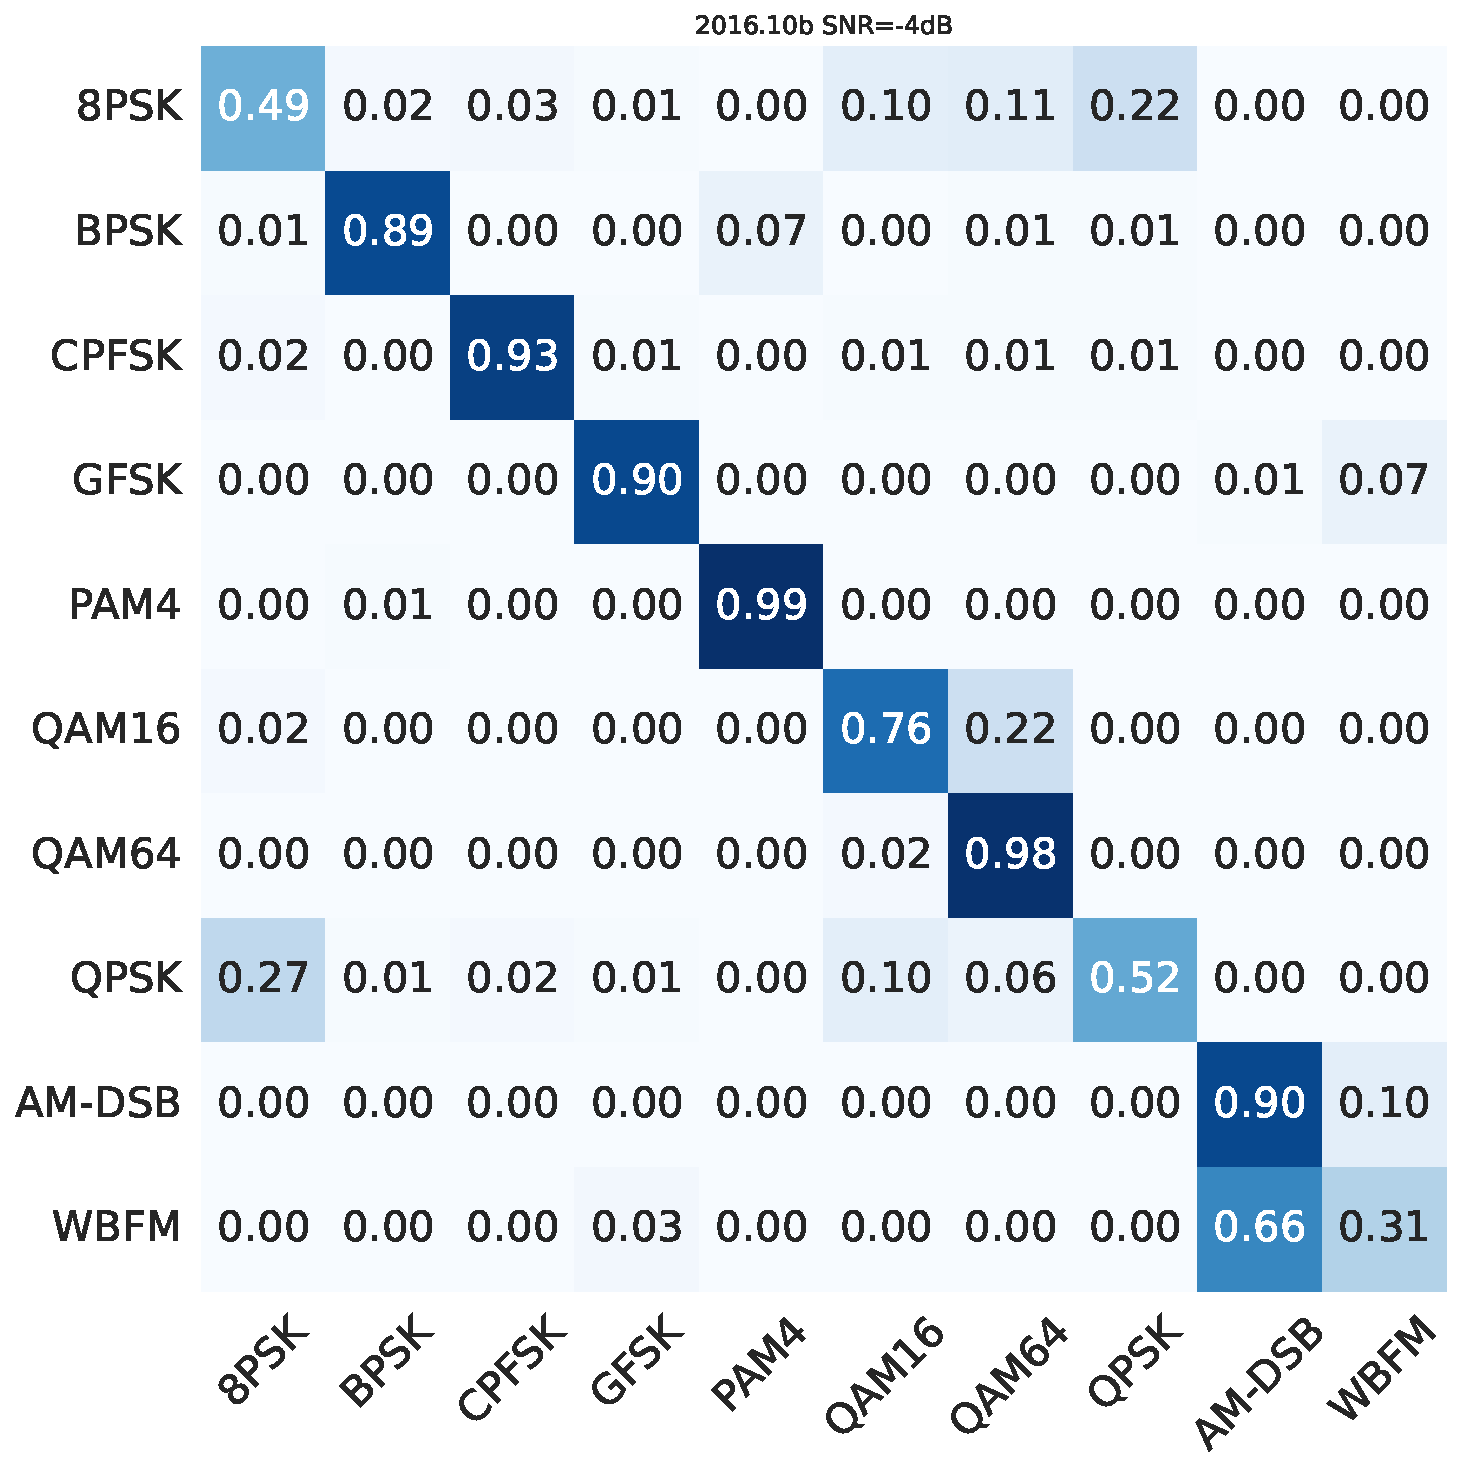
\includegraphics[width=0.24\linewidth]{Figures/IQFormerLite_RML201610B_confusionMatrix/2016.10b_-4.pdf}
				\hfill
				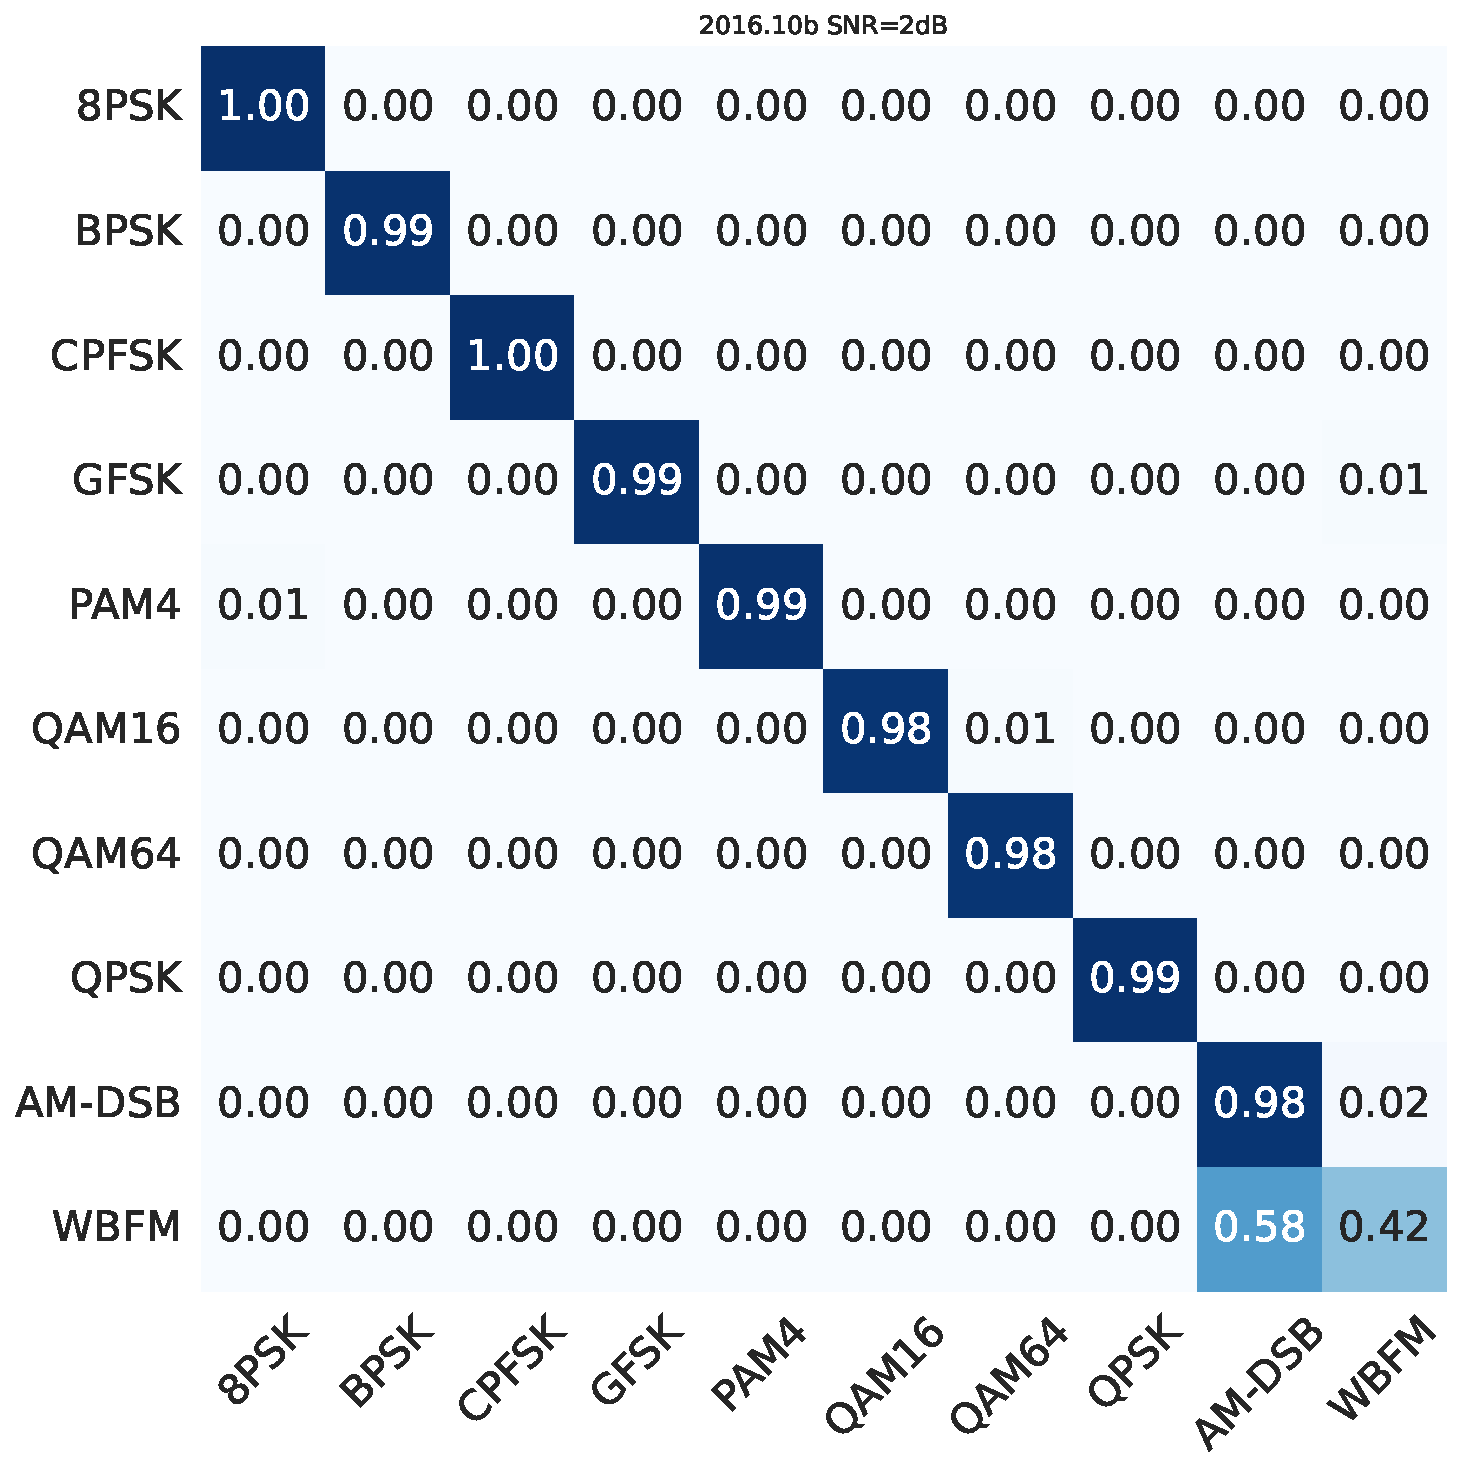
\includegraphics[width=0.24\linewidth]{Figures/IQFormerLite_RML201610B_confusionMatrix/2016.10b_2.pdf}
			}
		\end{adjustwidth}
		\caption{Confusion matrices of IQFormerLite under different SNR levels. For each dataset, the left matrix corresponds to SNR = -4 dB, and the right matrix corresponds to SNR = 2 dB. (a) Results on RadioML2016.10A. (b) Results on RadioML2016.10B. \label{fig:confusion_matrix}}
	\end{figure}
	
	\subsection{Ablation Study}
	To validate the LKF design, the ablation study evaluates three hyperparameters: grid size ($G$), grid range ($[-R, R]$), and kernel size ($K$).
	These parameters control the granularity and receptive field of the basis functions in Eq.~\eqref{eq:rbf}.
	The search space is $G \in \{2, 4, 8\}$, $[-R, R] \in \{[-1, 1], [-2, 2]\}$, and $K \in \{15, 17, 31\}$.
	
	Fig.~\ref{fig:kan_grid_ablation} shows that grid configuration and temporal receptive field jointly affect performance.
	The grid size $G$ shows a non-monotonic trend: increasing $G$ from 2 to 4 improves accuracy by capturing finer spectral variation, while increasing to $G=8$ degrades performance, likely due to overfitting or optimization instability.
	Expanding the grid range from $[-1, 1]$ to $[-2, 2]$ is beneficial, especially at $G=4$, because it better matches the distribution of normalized inputs $\mathbf{\hat{X}}$ and reduces boundary saturation.
	Kernel size $K$ also matters; larger kernels such as $K=31$ generally outperform smaller kernels such as $K=15$, providing a wider receptive field that is useful for low-frequency modulation cues.
	Based on these results, the default LKF configuration is $\{G=4, [-R, R]=[-2, 2], K=31\}$.
	
	\begin{figure}[htbp]
		\centering
		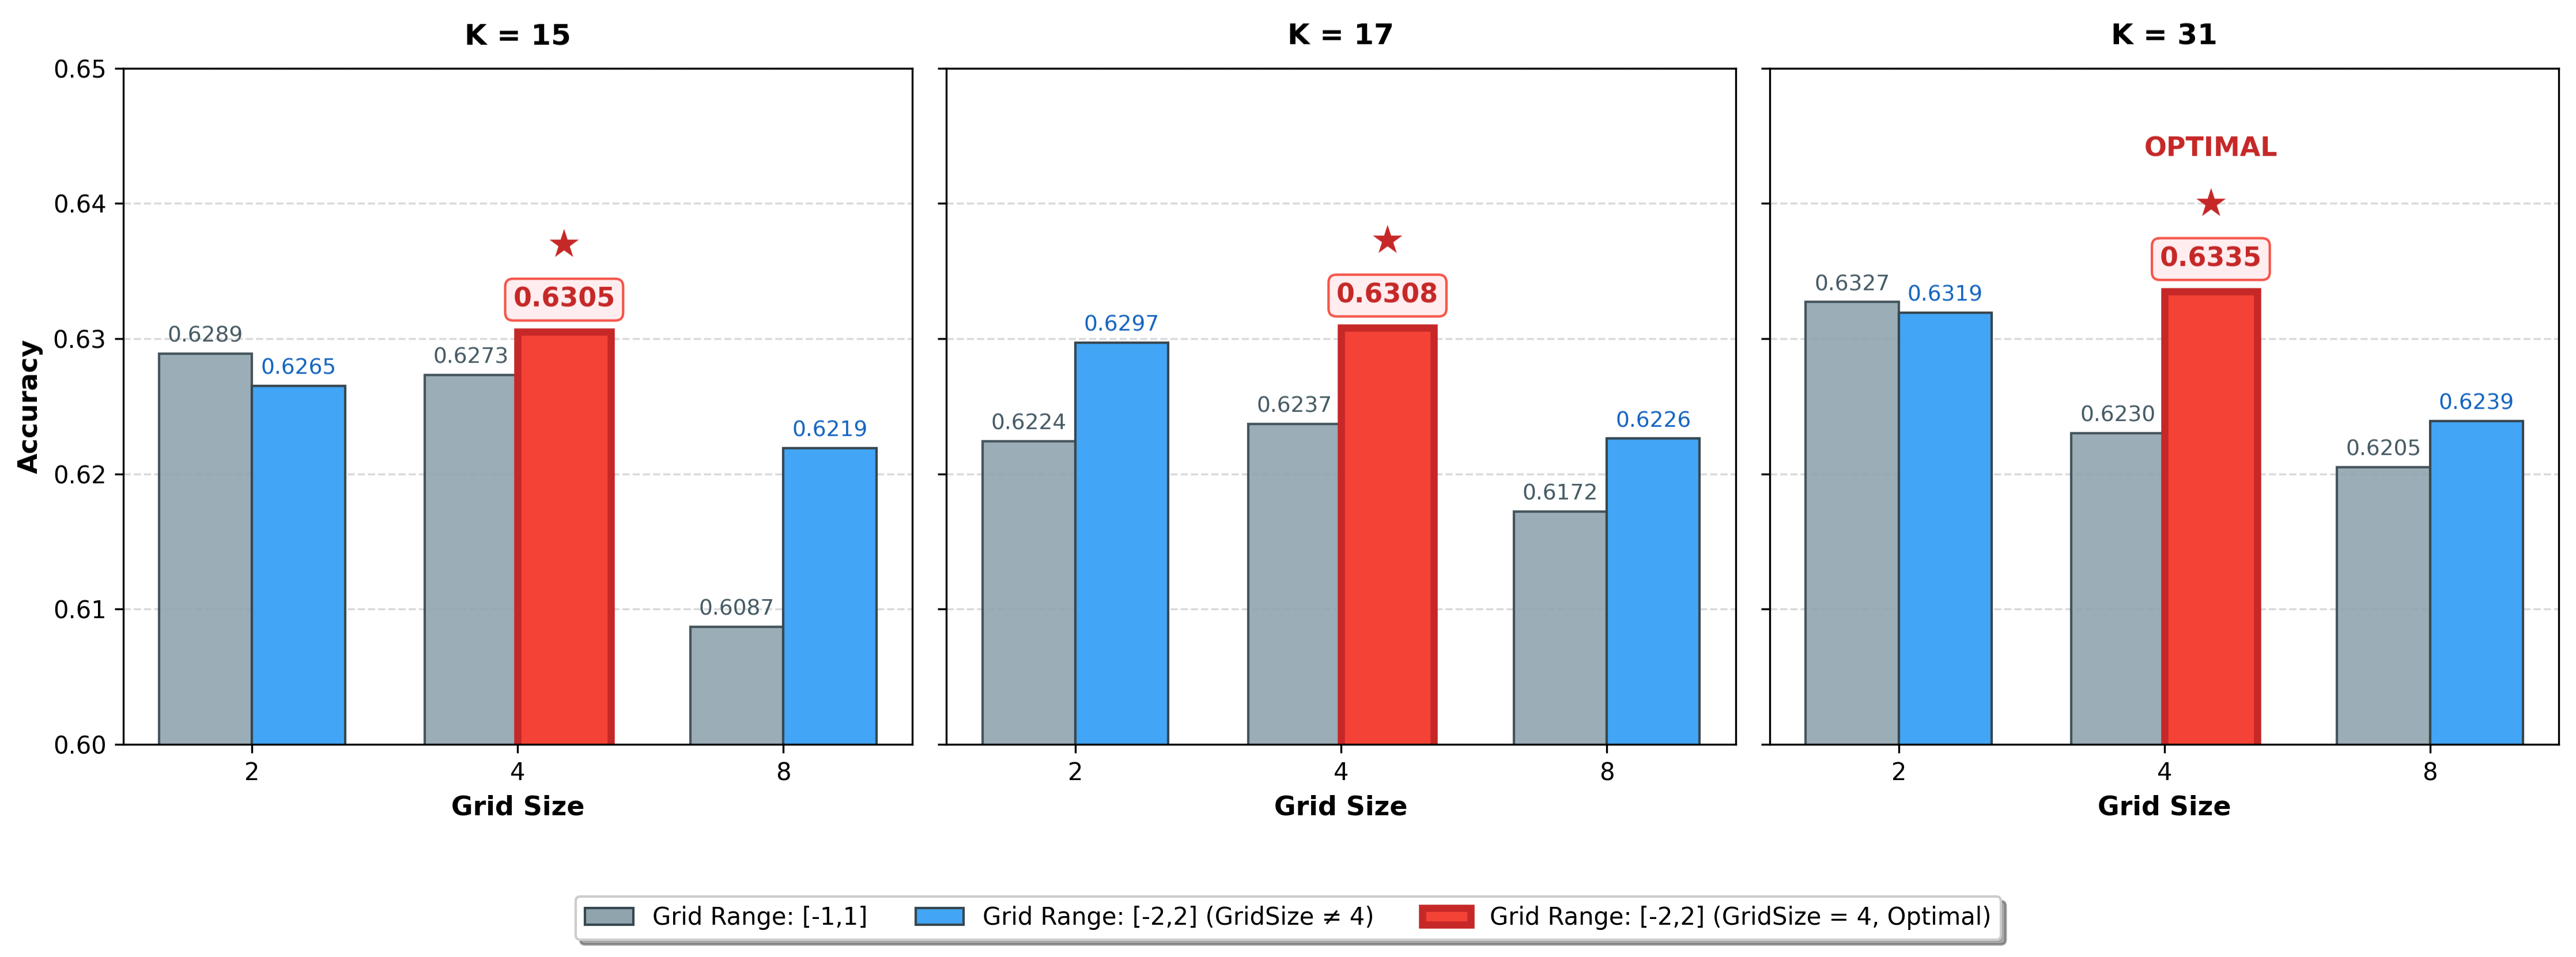
\includegraphics[width=0.98\linewidth]{Figures/kan_grid_ablation.png}
		\caption{Ablation results for the LKF module configuration. Accuracy is reported by varying the grid size $G$ and grid range $[-R, R]$ under three representative kernel sizes ($K \in \{15,17,31\}$). The optimal performance is achieved with the configuration $\{G=4, [-R, R]=[-2, 2], K=31\}$.}
		\label{fig:kan_grid_ablation}
	\end{figure}
	
	Following the selection of LKF hyperparameters, we performed component-level ablations to evaluate how each module affects the accuracy--efficiency trade-off. As summarized in Table~\ref{tab:ablation}, reducing the MLP blocks from 4 to 1 reveals substantial redundancy in the baseline feedforward design; parameters and computation are halved while accuracy drops by only 0.45\%. Further compression, including the removal of the LSTM and replacing EAA \cite{shaker2023SwiftFormerEfficient} with the LKGC module, reduces the parameter count to 0.11~M. While this aggressive optimization initially lowers accuracy to 62.00\%, the LKF module recovers this loss, improving overall accuracy by 1.35\% with negligible overhead.
	
	The final IQFormerLite architecture offers significant efficiency gains, reducing parameters by 65.7\% and FLOPs by 58.6\% compared to the original IQFormer. Despite using only about 34\% of the parameters and 41\% of the compute, IQFormerLite maintains an overall accuracy of 63.35\%, leaving a marginal gap of just 0.25 percentage points relative to the heavier baseline. these results suggest that combining LKGC and LKF effectively compensates for the absence of serial and attention-based operators.
	
%	\begin{table}[htbp]
%		\caption{Ablation study of different module designs on RML2016.10A. \label{tab:ablation}}
%		\renewcommand{\arraystretch}{1.2}
%		\begin{adjustwidth}{-\extralength}{0cm}
%			% 关键：最后三列改成 X X X，让它们更宽
%			\newcolumntype{Y}{>{\centering\arraybackslash}X} 
%			\begin{tabularx}{\fulllength}{l c c c c Y Y Y}
%				\toprule[1.5pt]
%				\textbf{Model} & \textbf{MLP Block} & \textbf{LSTM} & \textbf{Token Mixer} & \textbf{Filter Type} &
%				\textbf{Param. (M)} & \textbf{FLOPs (M)} & \textbf{Overall Acc. (\%)} \\
%				\midrule
%				
%				IQFormer (Baseline) & 4 & \checkmark & EAA & STFT & 0.35 & 77.48 & \textbf{63.60} \\
%				\mbox{w/o Large MLP} & 1 & \checkmark & EAA & STFT & 0.18 & 33.10 & 63.15 \\
%				w/o LSTM & 1 & $\times$ & EAA & STFT & 0.14 & 22.89 & 62.26 \\
%				with LKGC & 1 & $\times$ & LKGC & STFT & 0.11 & 28.54 & 62.00 \\
%				
%				\midrule
%				
%				\rowcolor{gray!15}
%				\textbf{IQFormerLite (Ours)} & \textbf{1} & \textbf{$\times$} & \textbf{LKGC} & \textbf{LKF} &
%				\textbf{0.12} (\textbf{$\downarrow 65.7\%$}) &
%				\textbf{32.06} (\textbf{$\downarrow 58.6\%$}) &
%				{63.35} ({$-0.25$}) \\
%				
%				\bottomrule[1.5pt]
%			\end{tabularx}
%		\end{adjustwidth}
%	\end{table}
	
%	\begin{table}[htbp]
%		\caption{Ablation study of different module designs on RML2016.10A.\label{tab:ablation}}
%		\renewcommand{\arraystretch}{1.15}
%		\begin{adjustwidth}{-\extralength}{0cm}
%			\centering
%			\setlength{\tabcolsep}{3.5pt} % 缩小列间距（关键）
%			% 可伸缩居中列（用于 tabularx 的 X）
%			\newcolumntype{Y}{>{\centering\arraybackslash}X}
%			% 定宽居中列（避免中间列抢宽）
%			\newcolumntype{P}[1]{>{\centering\arraybackslash}p{#1}}
%			
%			\begin{tabularx}{\linewidth}{X P{1.05cm} P{0.9cm} P{1.35cm} P{1.35cm} Y Y Y}
%				\toprule[1.5pt]
%				\textbf{Model} &
%				\textbf{MLP} &
%				\textbf{LSTM} &
%				\textbf{Token} &
%				\textbf{Filter} &
%				\makecell{\textbf{Param.}\\\textbf{(M)}} &
%				\makecell{\textbf{FLOPs}\\\textbf{(M)}} &
%				\makecell{\textbf{Overall}\\\textbf{(\%)}} \\
%				\midrule
%				
%				IQFormer  & 4 & \checkmark & EAA  & STFT & 0.35 & 77.48 & \textbf{63.60} \\
%				w/o Large MLP        & 1 & \checkmark & EAA  & STFT & 0.18 & 33.10 & 63.15 \\
%				w/o LSTM             & 1 & $\times$   & EAA  & STFT & 0.14 & 22.89 & 62.26 \\
%				with LKGC            & 1 & $\times$   & LKGC & STFT & 0.11 & 28.54 & 62.00 \\
%				\midrule
%				
%				\rowcolor{gray!15}
%				\textbf{Ours} & \textbf{1} & \textbf{$\times$} & \textbf{LKGC} & \textbf{LKF} &
%				\makecell{\textbf{0.12}\\(\textbf{$\downarrow 65.7\%$})} &
%				\makecell{\textbf{32.06}\\(\textbf{$\downarrow 58.6\%$})} &
%				\makecell{63.35\\($-0.25$)} \\
%				\bottomrule[1.5pt]
%			\end{tabularx}
%		\end{adjustwidth}
%	\end{table}
	
	\begin{table}[htbp]
		\caption{Ablation study of different module designs on RML2016.10A.\label{tab:ablation}}
		\renewcommand{\arraystretch}{1.15}
		\begin{adjustwidth}{-\extralength}{0cm}
			\centering
			\setlength{\tabcolsep}{3.5pt} % 缩小列间距（关键）
			
			% 定义带有相对宽度比例的列类型
			% 第一列（宽）：分配 1.3 倍的 X 宽度
			\newcolumntype{L}{>{\hsize=1.3\hsize\raggedright\arraybackslash}X}
			% 最后三列（窄）：各分配 0.9 倍的 X 宽度
			\newcolumntype{Y}{>{\hsize=0.9\hsize\centering\arraybackslash}X}
			
			% 定宽居中列（避免中间列抢宽）
			\newcolumntype{P}[1]{>{\centering\arraybackslash}p{#1}}
			
			% 注意第一列改成了我们新定义的 L
			\begin{tabularx}{\linewidth}{L P{1.05cm} P{0.9cm} P{1.35cm} P{1.35cm} Y Y Y}
				\toprule[1.5pt]
				\textbf{Model} &
				\textbf{MLP} &
				\textbf{LSTM} &
				\textbf{Token} &
				\textbf{Filter} &
				\makecell{\textbf{Param.}\\\textbf{(M)}} &
				\makecell{\textbf{FLOPs}\\\textbf{(M)}} &
				\makecell{\textbf{Overall}\\\textbf{(\%)}} \\
				\midrule
				
				IQFormer  & 4 & \checkmark & EAA  & STFT & 0.35 & 77.48 & \textbf{63.60} \\
				w/o Large MLP        & 1 & \checkmark & EAA  & STFT & 0.18 & 33.10 & 63.15 \\
				w/o LSTM             & 1 & $\times$   & EAA  & STFT & 0.14 & 22.89 & 62.26 \\
				with LKGC            & 1 & $\times$   & LKGC & STFT & 0.11 & 28.54 & 62.00 \\
				\midrule
				
				\rowcolor{gray!15}
				\textbf{Ours} & \textbf{1} & \textbf{$\times$} & \textbf{LKGC} & \textbf{LKF} &
				\makecell{\textbf{0.12}\\(\textbf{$\downarrow 65.7\%$})} &
				\makecell{\textbf{32.06}\\(\textbf{$\downarrow 58.6\%$})} &
				\makecell{63.35\\($-0.25$)} \\
				\bottomrule[1.5pt]
			\end{tabularx}
		\end{adjustwidth}
	\end{table}
	
	\subsection{Visualization Analysis}
	Fig.~\ref{fig:tsne_vis} illustrates how feature separability changes with signal quality.
	At SNR $=-12$~dB (left column), embeddings from different modulation types are widely mixed, which indicates that noise dominates and class structure is difficult to recover.
	At SNR $=0$~dB (middle column), embeddings begin to form class-related regions and several categories become more distinct, although boundaries remain diffuse and overlap persists.
	At SNR $=12$~dB (right column), most classes form compact and well-separated clusters, reflecting stronger discriminative structure as the noise floor decreases.
	AM-DSB and WBFM still overlap at $12$~dB, which is consistent with the confusion observed in the quantitative results.
	
	\begin{figure}[htbp]
		\begin{adjustwidth}{-\extralength}{0cm}
			\centering
			
			\subfloat[\centering  RadioML2016.10A\label{fig:tsne_a}]{
				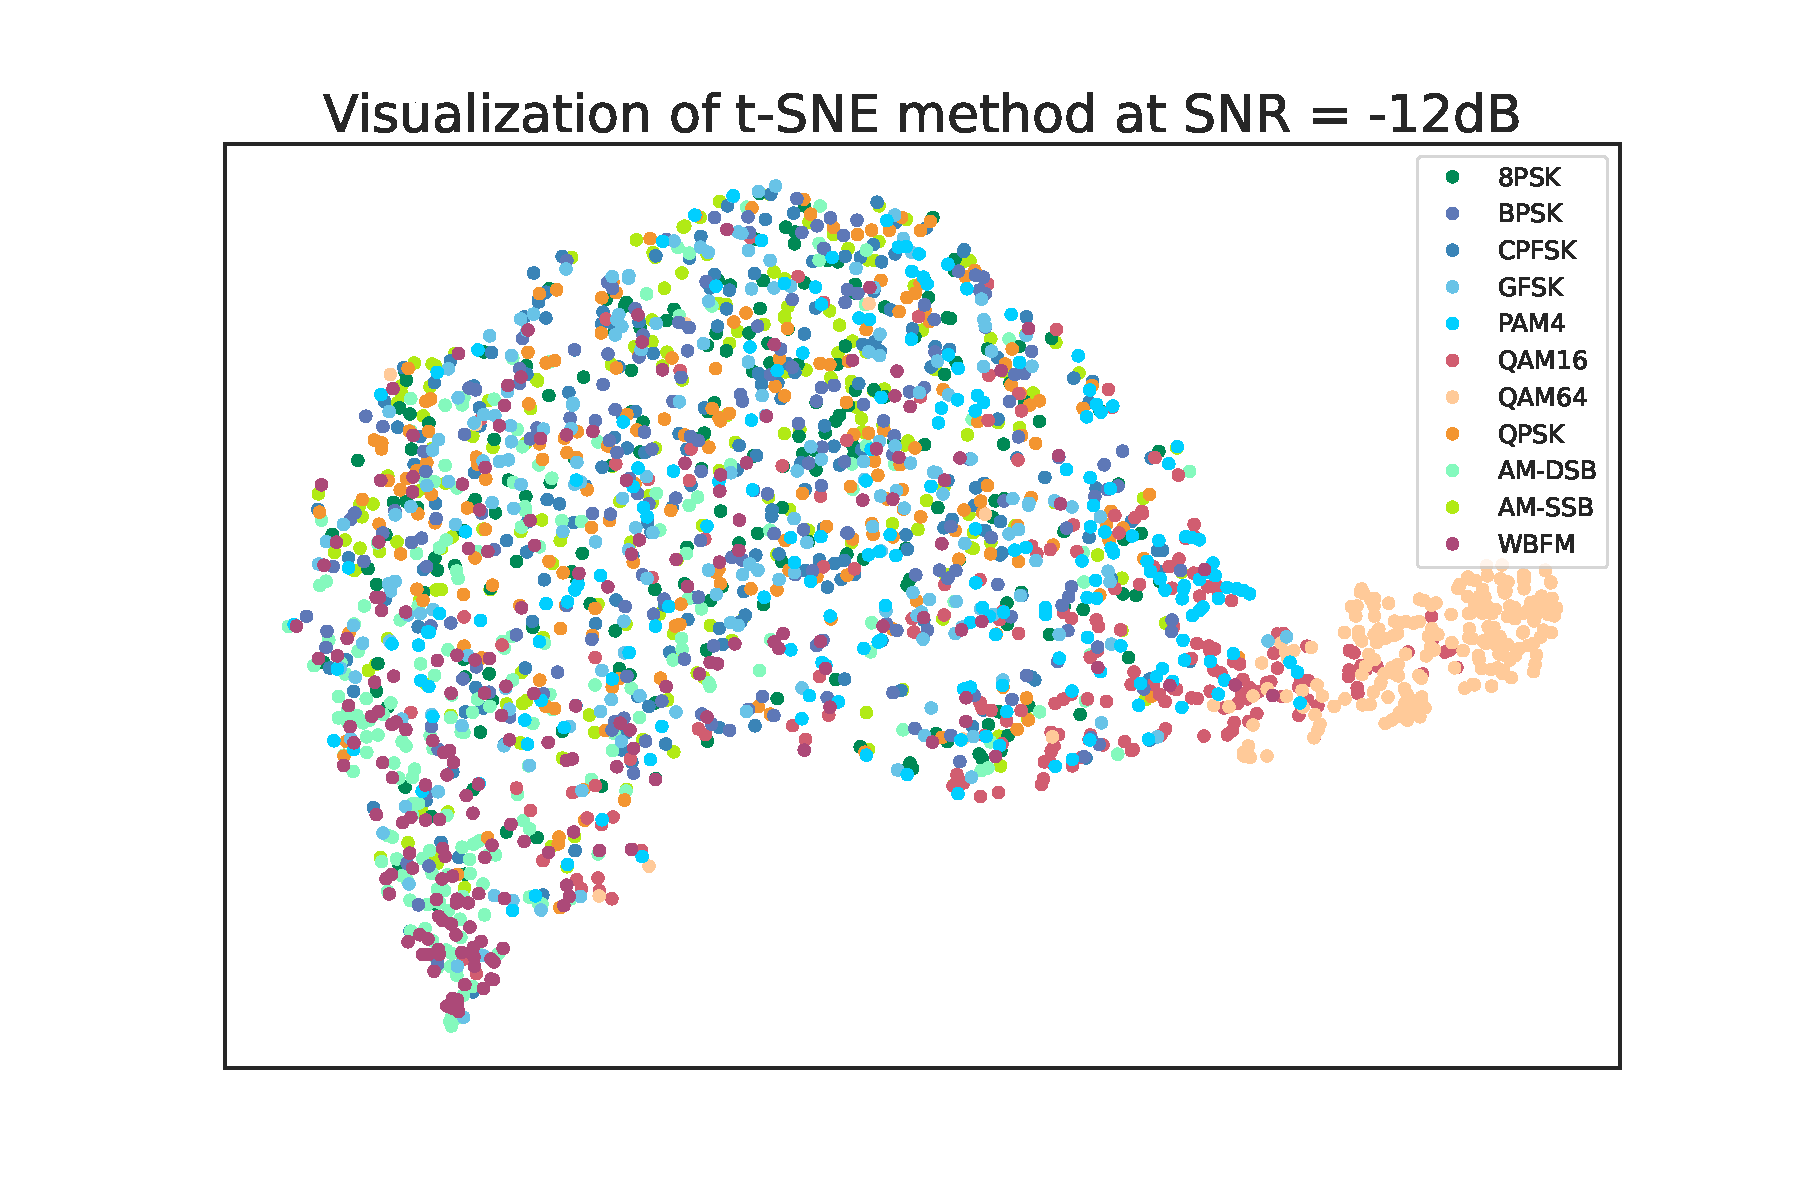
\includegraphics[width=0.32\linewidth]{Figures/IQFormerLite_RML201610A_tsne/tsne_2016.10a_-12.pdf}
				\hfill
				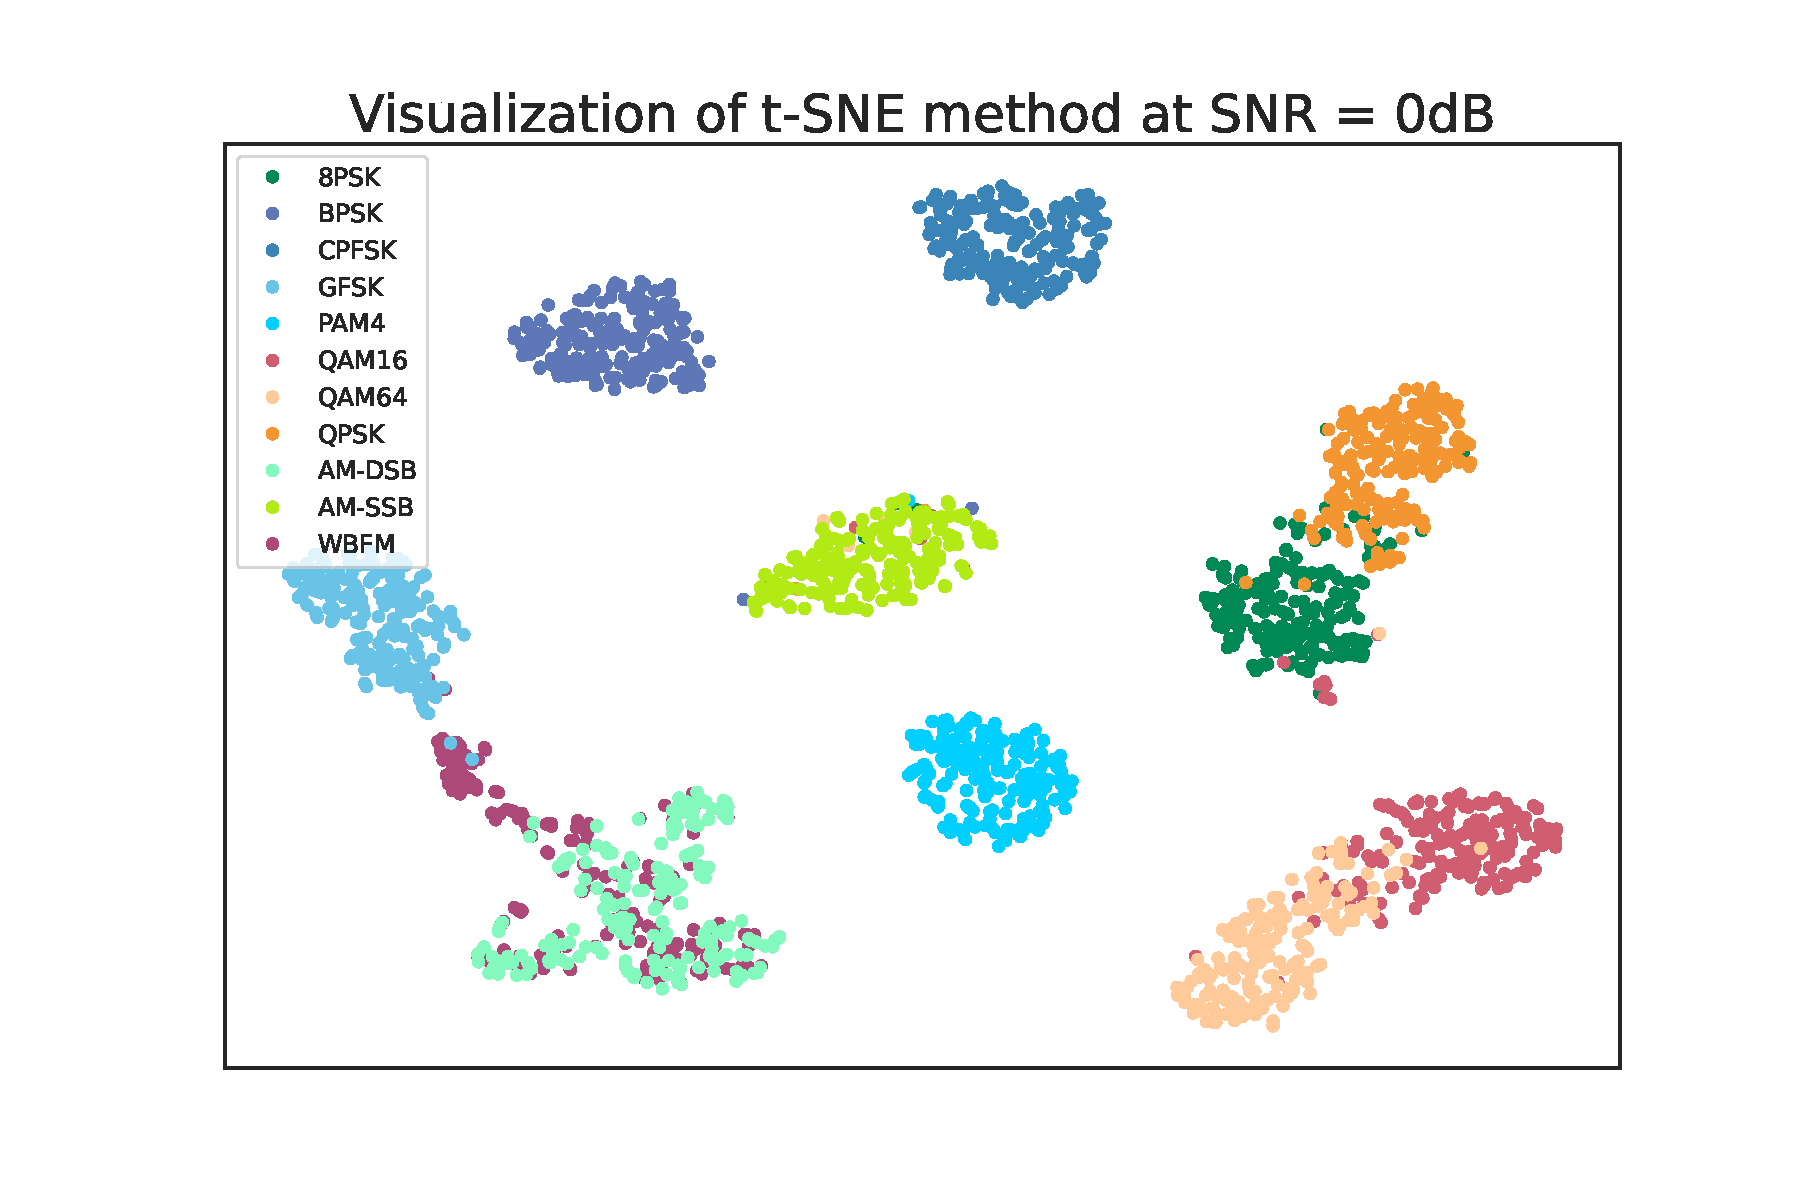
\includegraphics[width=0.32\linewidth]{Figures/IQFormerLite_RML201610A_tsne/tsne_2016.10a_0.pdf}
				\hfill
				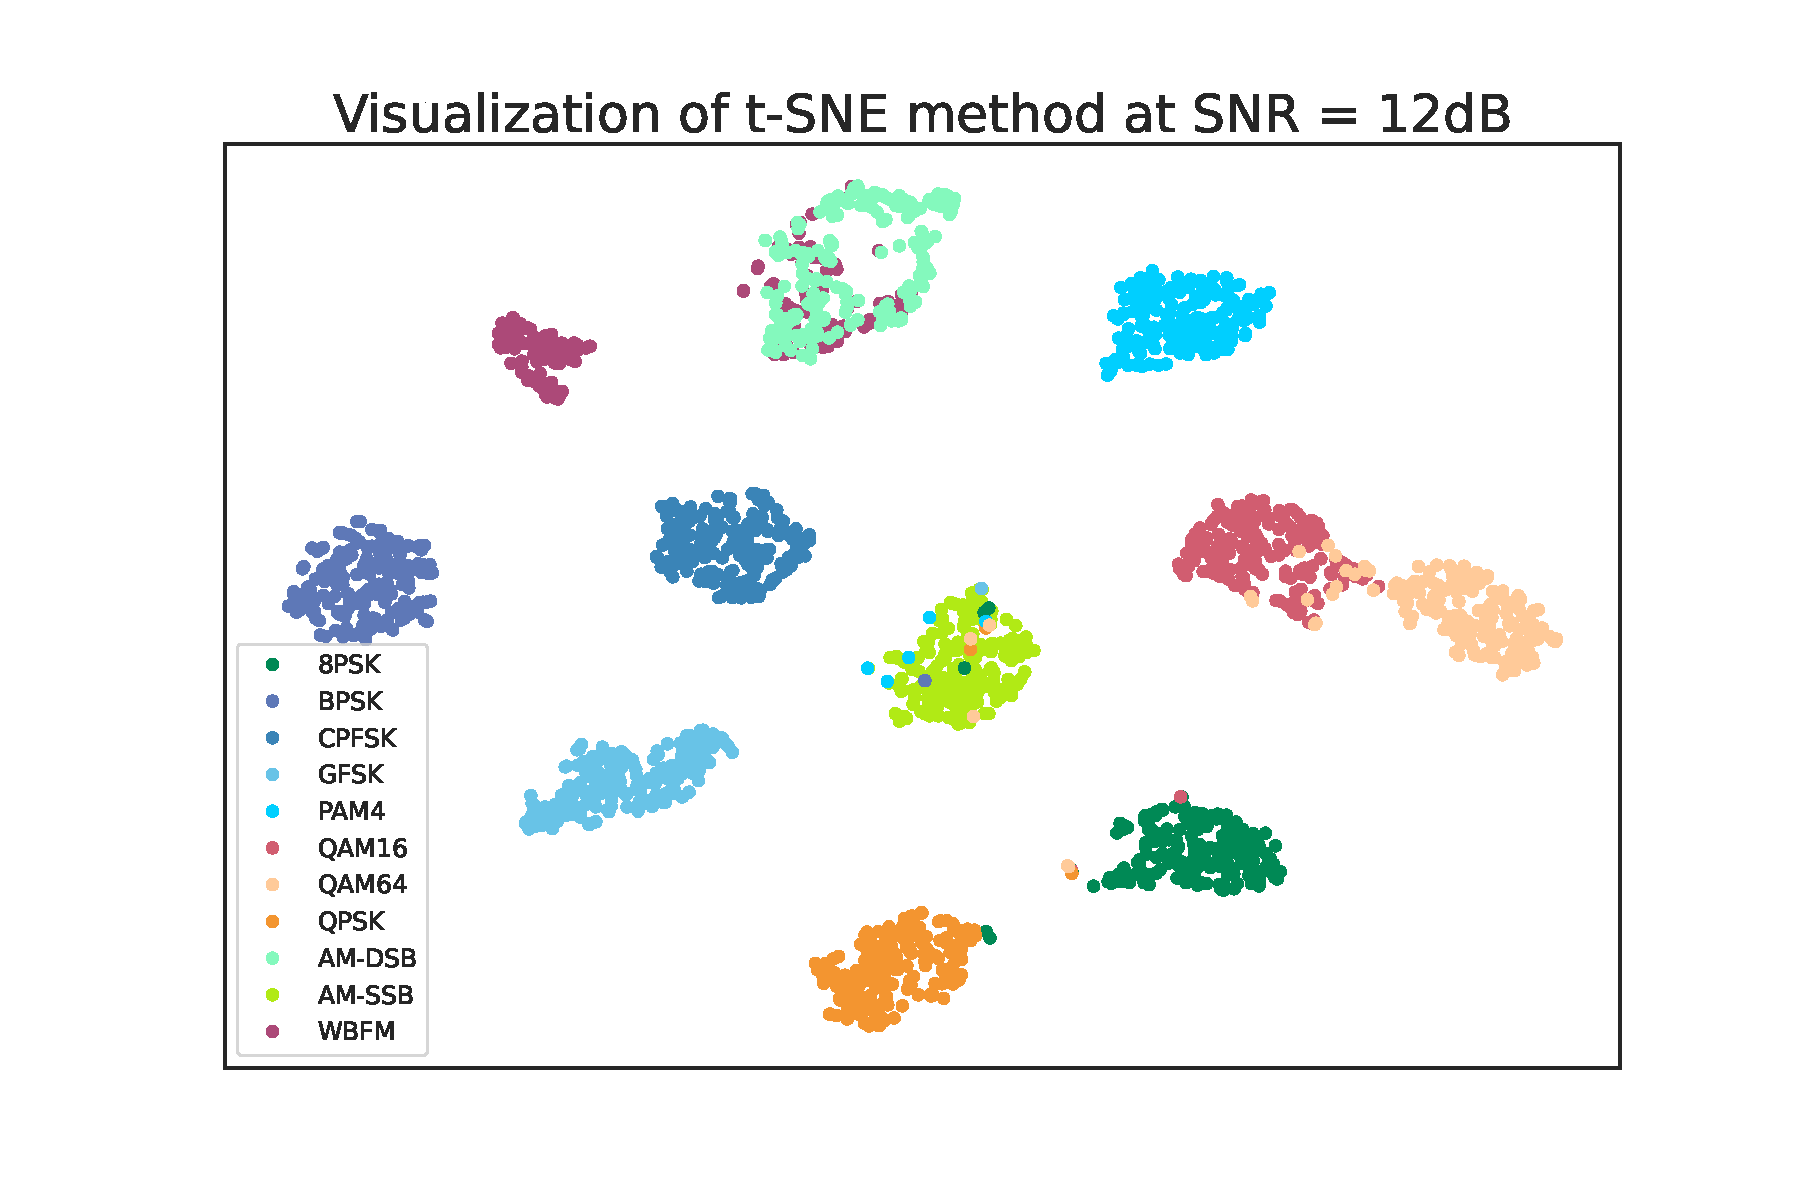
\includegraphics[width=0.32\linewidth]{Figures/IQFormerLite_RML201610A_tsne/tsne_2016.10a_12.pdf}
			}
			
			\subfloat[\centering RadioML2016.10B\label{fig:tsne_b}]{
				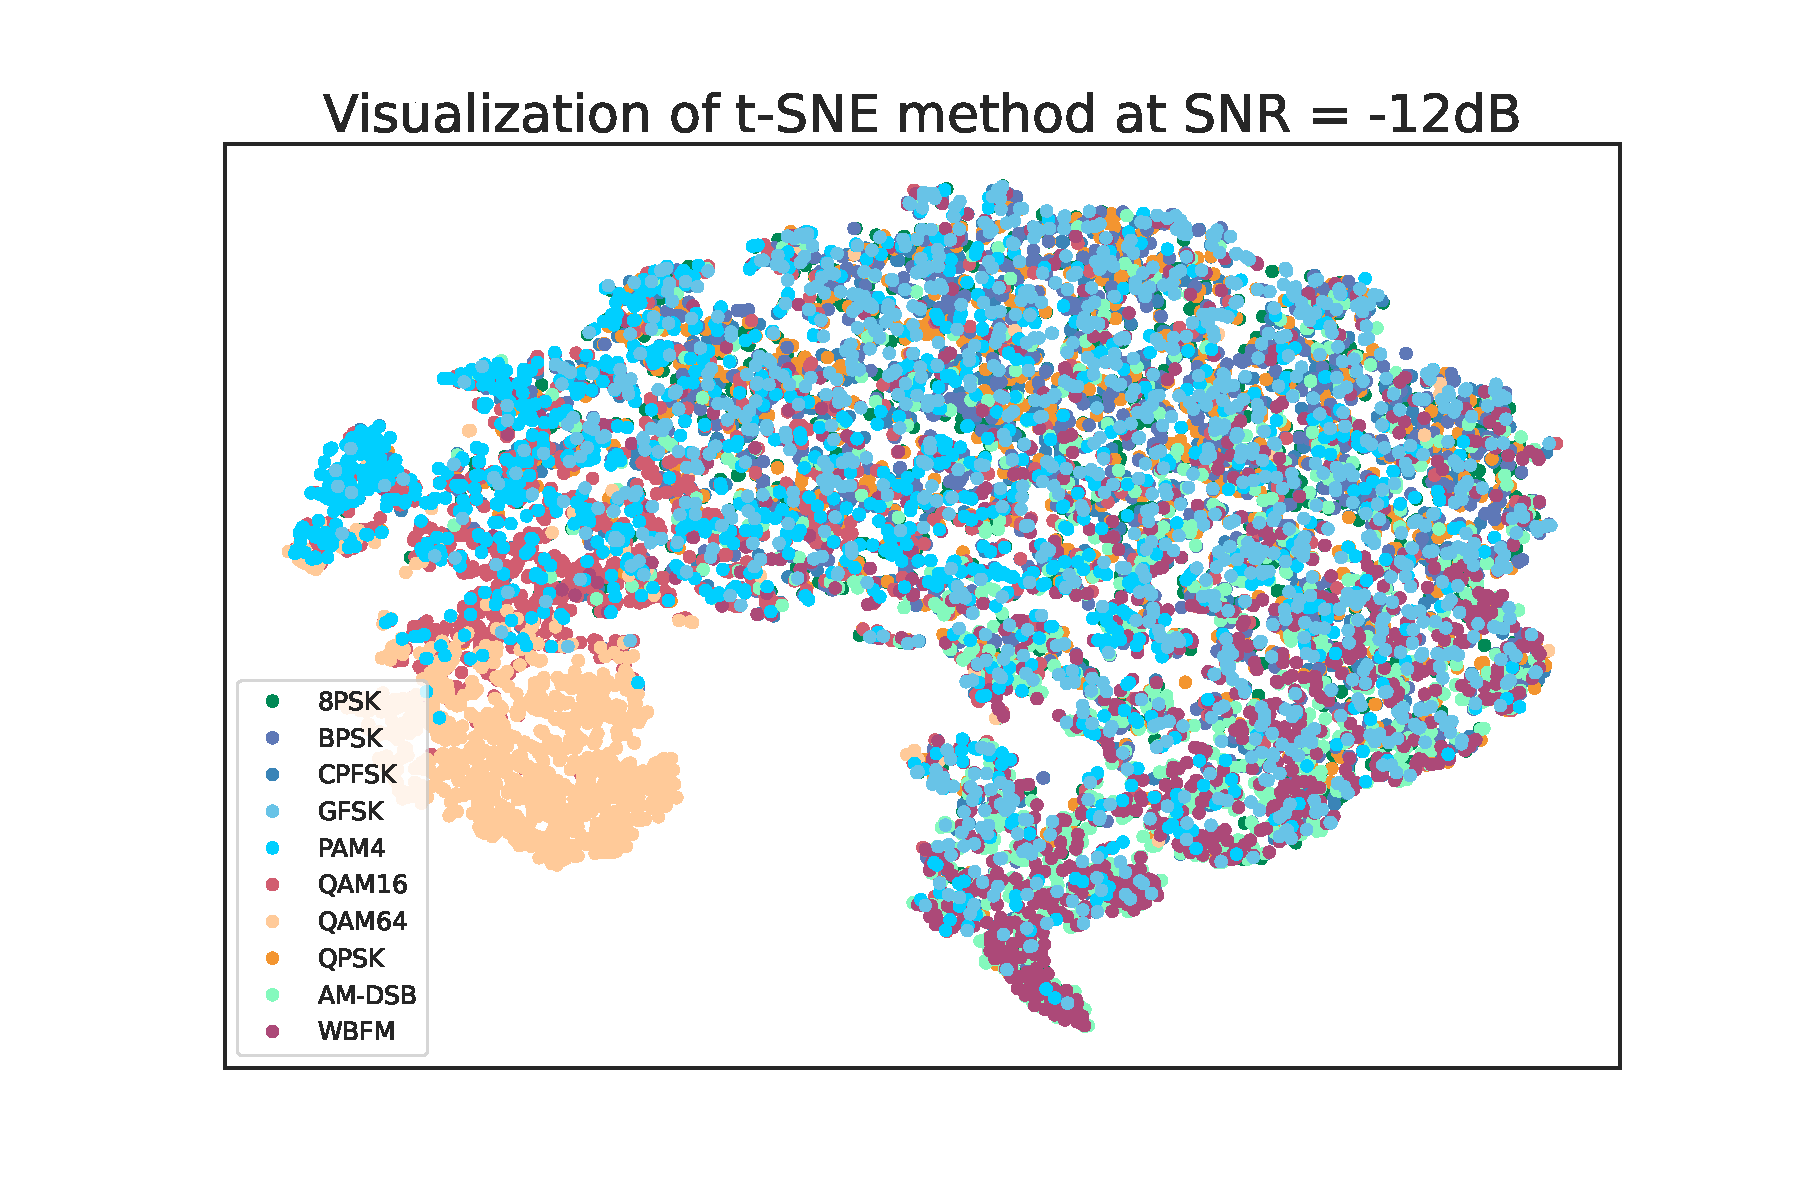
\includegraphics[width=0.32\linewidth]{Figures/IQFormerLite_RML201610B_tsne/tsne_2016.10b_-12.pdf}
				\hfill
				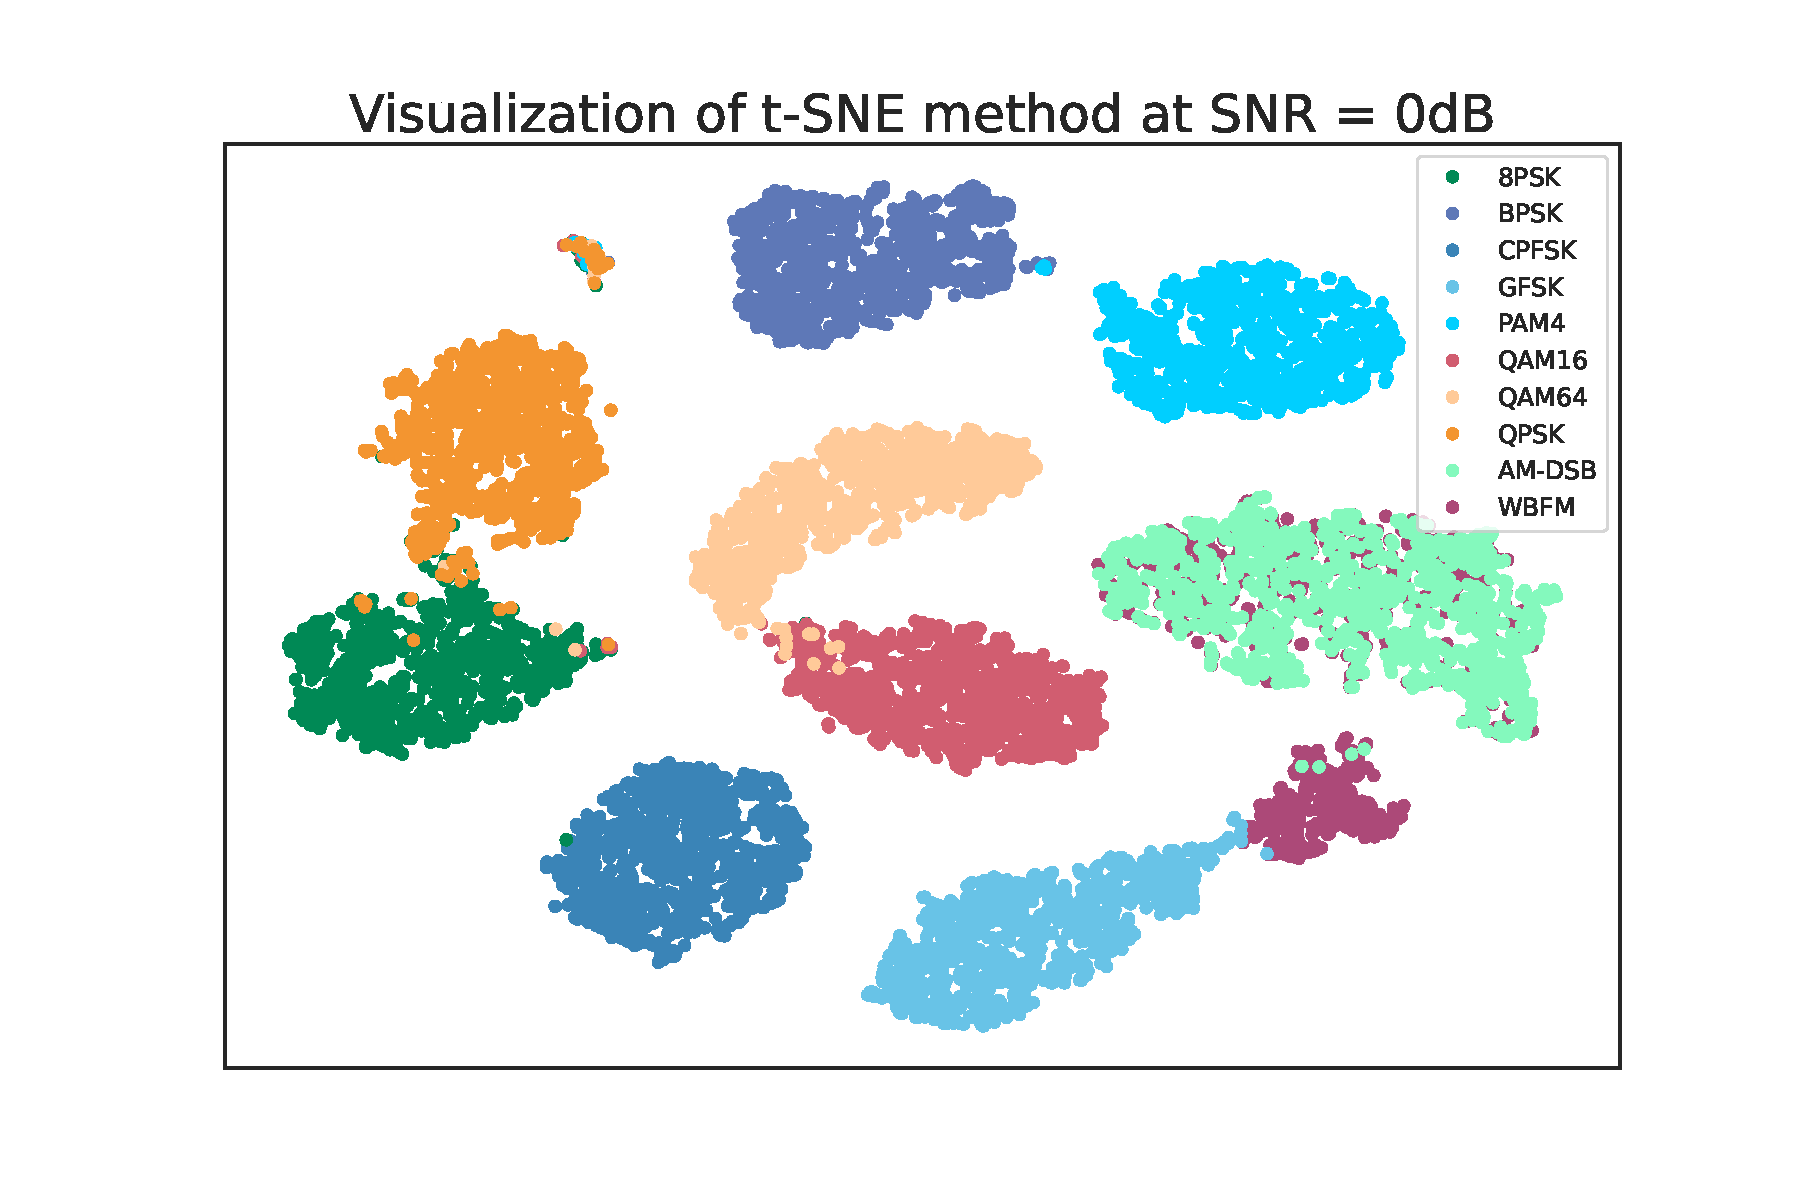
\includegraphics[width=0.32\linewidth]{Figures/IQFormerLite_RML201610B_tsne/tsne_2016.10b_0.pdf}
				\hfill
				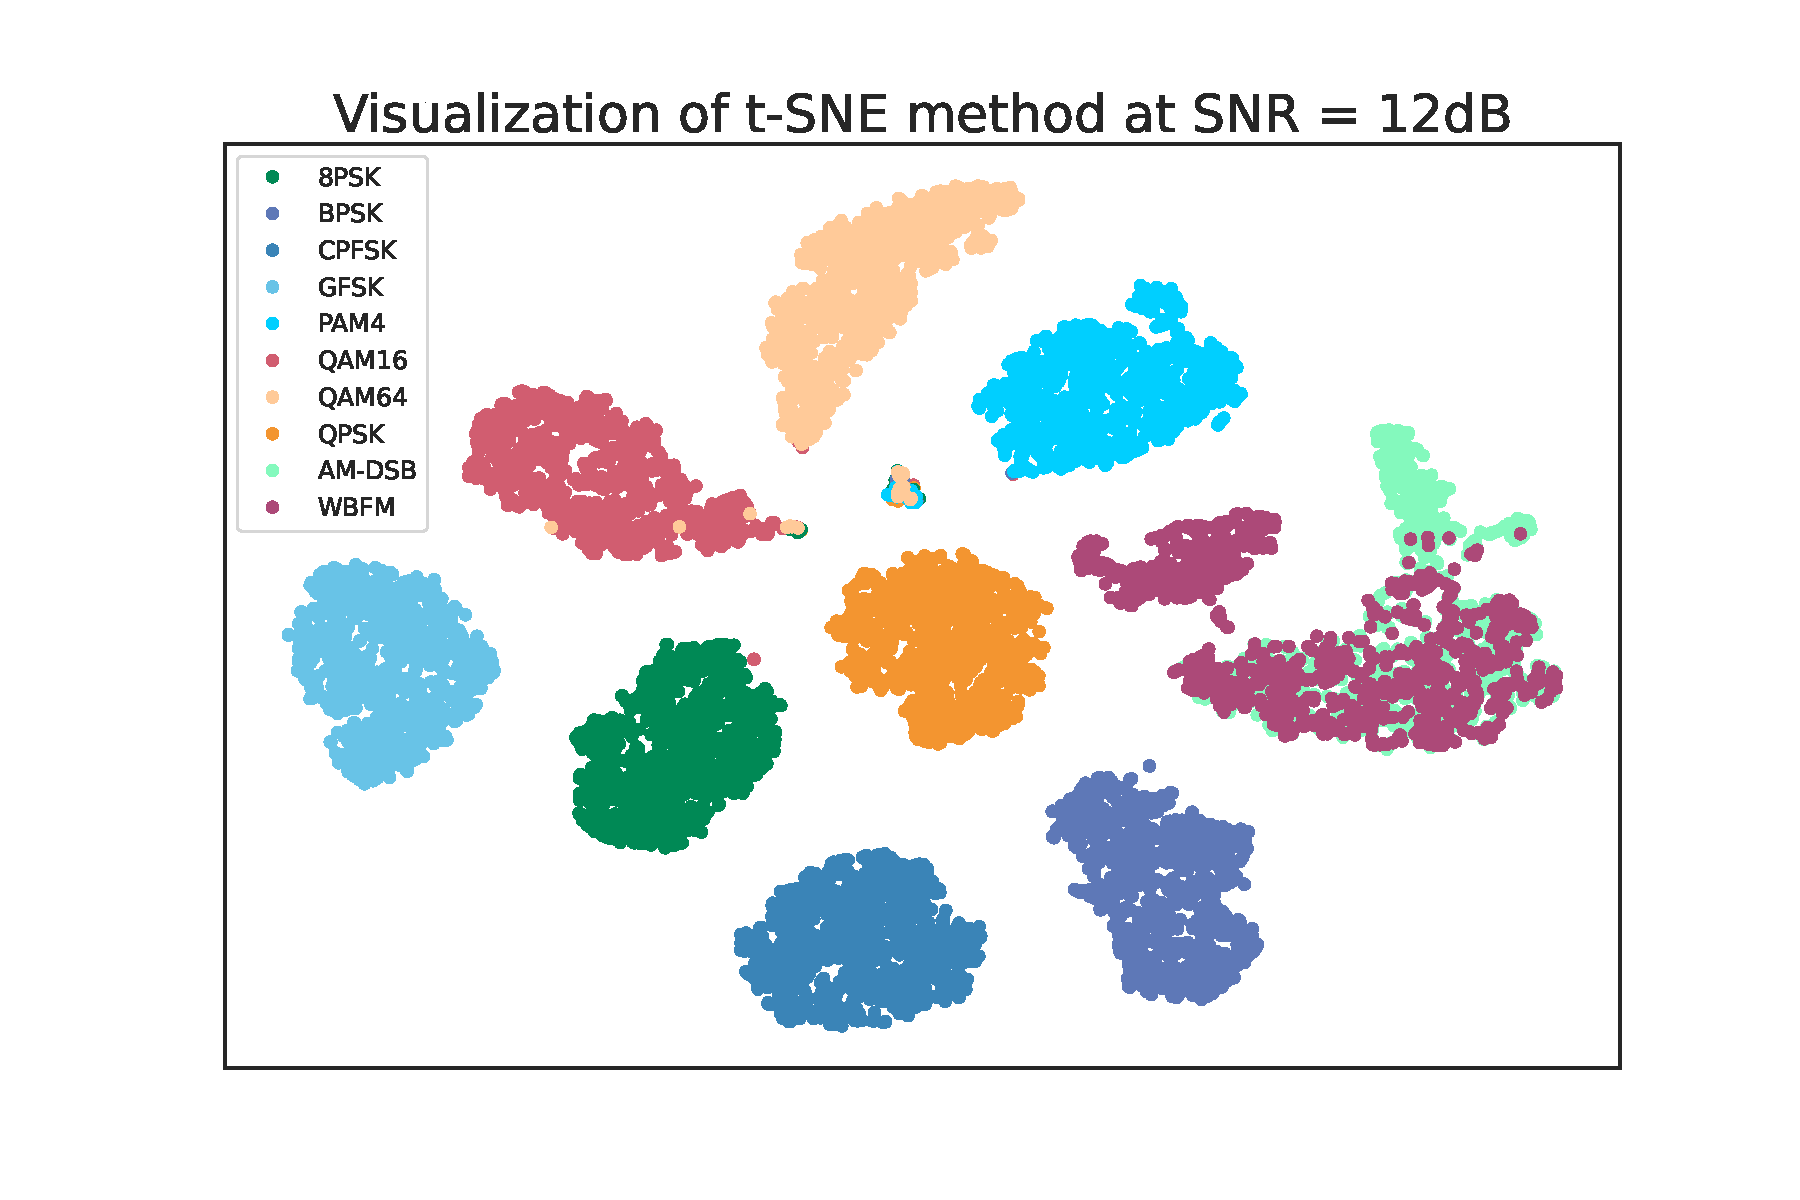
\includegraphics[width=0.32\linewidth]{Figures/IQFormerLite_RML201610B_tsne/tsne_2016.10b_12.pdf}
			}
			
		\end{adjustwidth}
		\caption{t-SNE visualization of feature representations under varying SNR levels. From left to right, the columns correspond to SNR = -20 dB, -6 dB, and 12 dB. (a) Results on RadioML2016.10A. (b) Results on RadioML2016.10B. \label{fig:tsne_vis}}
	\end{figure}
	
	\subsection{Deployment Efficiency on Edge NPU}
	\label{sec:deployment}
	
	This section reports on-device measurements of IQFormerLite on the Rockchip RK3588 platform. We profile latency, throughput, and memory overhead after compiling the models with RKNN-Toolkit2 into FP32, FP16, and INT8.
	
	Table~\ref{tab:quant_npu} shows that IQFormerLite is consistently more efficient than the baseline IQFormer across all formats. Under FP32, the compiled RKNN size drops from 4261.38~KB to 909.10~KB (78.7\%), while latency decreases from 2.30~ms to 0.20~ms (91.3\%). These reductions translate into an $11.45\times$ throughput increase, from 435.23 to 4983.30~samples/s. The gap is even larger in INT8, where IQFormerLite reaches 5877.30~samples/s, corresponding to a $13.46\times$ increase over the baseline. IQFormerLite also operates at lower NPU load (48\%--49\%) than IQFormer (79\%), suggesting that its operator mix maps more effectively to the RK3588 NPU kernels on this deployment stack.
	
%	\begin{table*}[t]
%		%		\caption{On-device performance under different quantization levels across multiple metrics. \label{tab:quant_npu}}
%		%		\caption{On-device performance of IQFormer and IQFormerLite on the Rockchip RK3588 NPU under different quantization types. Quant. denotes the quantization type used for RKNN compilation. {$\Delta$Mem (MB)} indicates activation memory (runtime RAM overhead). {Lat. (ms)} is per-sample inference latency, and {Thr. (samples/s)} is throughput. \label{tab:quant_npu}}
%		\caption{On-device performance of IQFormer and IQFormerLite on the Rockchip RK3588 NPU under different quantization types. Quant. \textasciitilde  quantization type; {$\Delta$Mem} \textasciitilde activation memory (runtime RAM overhead); Lat. \textasciitilde per-sample inference latency; Thr. \textasciitilde throughput. \label{tab:quant_npu}}
%		
%		
%		\renewcommand{\arraystretch}{1.2}
%		\small
%		\sisetup{
%			table-number-alignment = center,
%			detect-weight = true,
%			round-mode = places,
%			round-precision = 2
%		}
%		\begin{adjustwidth}{-\extralength}{0cm}
%			\newcolumntype{Y}{>{\centering\arraybackslash}X}
%			\begin{tabularx}{\fulllength}{l l Y Y Y Y Y Y}
%				\toprule
%				\multirow{2}{*}{\textbf{Quant.}} & \multirow{2}{*}{\textbf{Method}} &
%				\multicolumn{2}{c}{\textbf{Footprint}} &
%				\multicolumn{2}{c}{\textbf{Runtime}} &
%				\textbf{Util.} & \textbf{Quality} \\
%				\cmidrule(lr){3-4} \cmidrule(lr){5-6} \cmidrule(lr){7-7} \cmidrule(lr){8-8}
%				& & {Size (KB)} & {$\Delta$Mem (MB)} & {Lat. (ms)} & {Thr. (samples/s)} & {NPU Load (\%)} & {Acc. (\%)} \\
%				\midrule
%				
%				\multirow{3}{*}{FP32}
%				& IQFormer & 4261.38 & 12.3 & 2.30 & 435.23 & 79 & 62.03 \\
%				%				\rowcolor{gray!10}
%				& \textbf{IQFormerLite} & \textbf{909.10} & \textbf{7.6} & \textbf{0.20} & \textbf{4983.30} & \textbf{49} & \textbf{66.20} \\
%				& \textit{Gain (Lite vs. Base)} & {\textit{$\downarrow$78.7\%}} & {\textit{$\downarrow$38.2\%}} & {\textit{$\downarrow$91.3\%}} & {\textit{$\times$11.45}} & {\textit{$\downarrow$38.0\%}} & {\textit{$+4.17$ pp}} \\
%				\midrule
%				
%				\multirow{3}{*}{FP16}
%				& IQFormer & 4261.38 & 12.5 & 2.29 & 435.10 & 79 & 62.03 \\
%				%				\rowcolor{gray!10}
%				& \textbf{IQFormerLite} & \textbf{909.10} & \textbf{5.3} & \textbf{0.21} & \textbf{4836.20} & \textbf{48} & \textbf{66.00} \\
%				& \textit{Gain (Lite vs. Base)} & {\textit{$\downarrow$78.7\%}} & {\textit{$\downarrow$57.6\%}} & {\textit{$\downarrow$90.8\%}} & {\textit{$\times$11.12}} & {\textit{$\downarrow$39.2\%}} & {\textit{$+3.97$ pp}} \\
%				\midrule
%				
%				\multirow{3}{*}{INT8}
%				& IQFormer & 4046.92 & 11.9 & 2.28 & 436.69 & 79 & 54.32 \\
%				%				\rowcolor{gray!10}
%				& \textbf{IQFormerLite} & \textbf{735.38} & \textbf{0.9} & \textbf{0.17} & \textbf{5877.30} & \textbf{48} & \textbf{65.80} \\
%				& \textit{Gain (Lite vs. Base)} & {\textit{$\downarrow$81.8\%}} & {\textit{$\downarrow$92.4\%}} & {\textit{$\downarrow$92.5\%}} & {\textit{$\times$13.46}} & {\textit{$\downarrow$39.2\%}} & {\textit{$+11.48$ pp}} \\
%				\bottomrule
%			\end{tabularx}
%		\end{adjustwidth}
%	\end{table*}
	
	\begin{table}[htbp]
		\caption{On-device performance of IQFormer and IQFormerLite on the Rockchip RK3588 NPU under different quantization types. Quant. \textasciitilde  quantization type; {$\Delta$Mem} \textasciitilde activation memory (runtime RAM overhead); Lat. \textasciitilde per-sample inference latency; Thr. \textasciitilde throughput. \label{tab:quant_npu}}
		
		\renewcommand{\arraystretch}{1.2}
		\small
		\centering % 添加居中命令
		\sisetup{
			table-number-alignment = center,
			detect-weight = true,
			round-mode = places,
			round-precision = 2
		}
		
		% 定义 Y 为居中且自适应宽度的列
		\newcolumntype{Y}{>{\centering\arraybackslash}X}
		
		% 将 \fulllength 替换为 \textwidth，并去除了 adjustwidth 环境
		\begin{tabularx}{\textwidth}{l l Y Y Y Y Y Y}
			\toprule
			\multirow{2}{*}{\textbf{Quant.}} & \multirow{2}{*}{\textbf{Method}} &
			\multicolumn{2}{c}{\textbf{Footprint}} &
			\multicolumn{2}{c}{\textbf{Runtime}} &
			\textbf{Util.} & \textbf{Quality} \\
			\cmidrule(lr){3-4} \cmidrule(lr){5-6} \cmidrule(lr){7-7} \cmidrule(lr){8-8}
			& & {Size (KB)} & {$\Delta$Mem (MB)} & {Lat. (ms)} & {Thr. (samples/s)} & {NPU Load (\%)} & {Acc. (\%)} \\
			\midrule
			
			\multirow{3}{*}{FP32}
			& IQFormer & 4261.38 & 12.3 & 2.30 & 435.23 & 79 & 62.03 \\
			& \textbf{IQFormerLite} & \textbf{909.10} & \textbf{7.6} & \textbf{0.20} & \textbf{4983.30} & \textbf{49} & \textbf{66.20} \\
			& \textit{Gain (Lite vs. Base)} & {\textit{$\downarrow$78.7\%}} & {\textit{$\downarrow$38.2\%}} & {\textit{$\downarrow$91.3\%}} & {\textit{$\times$11.45}} & {\textit{$\downarrow$38.0\%}} & {\textit{$+4.17$ pp}} \\
			\midrule
			
			\multirow{3}{*}{FP16}
			& IQFormer & 4261.38 & 12.5 & 2.29 & 435.10 & 79 & 62.03 \\
			& \textbf{IQFormerLite} & \textbf{909.10} & \textbf{5.3} & \textbf{0.21} & \textbf{4836.20} & \textbf{48} & \textbf{66.00} \\
			& \textit{Gain (Lite vs. Base)} & {\textit{$\downarrow$78.7\%}} & {\textit{$\downarrow$57.6\%}} & {\textit{$\downarrow$90.8\%}} & {\textit{$\times$11.12}} & {\textit{$\downarrow$39.2\%}} & {\textit{$+3.97$ pp}} \\
			\midrule
			
			\multirow{3}{*}{INT8}
			& IQFormer & 4046.92 & 11.9 & 2.28 & 436.69 & 79 & 54.32 \\
			& \textbf{IQFormerLite} & \textbf{735.38} & \textbf{0.9} & \textbf{0.17} & \textbf{5877.30} & \textbf{48} & \textbf{65.80} \\
			& \textit{Gain (Lite vs. Base)} & {\textit{$\downarrow$81.8\%}} & {\textit{$\downarrow$92.4\%}} & {\textit{$\downarrow$92.5\%}} & {\textit{$\times$13.46}} & {\textit{$\downarrow$39.2\%}} & {\textit{$+11.48$ pp}} \\
			\bottomrule
		\end{tabularx}
	\end{table}
	
	IQFormerLite is also stable under post-training quantization on this platform. Moving from FP32 to INT8 reduces accuracy from 66.20\% to 65.80\%, a 0.40 percentage-point change, whereas IQFormer drops from 62.03\% to 54.32\% (7.71 percentage points). INT8 further reduces IQFormerLite's incremental runtime memory to 0.9~MB, compared with 11.9~MB for the baseline under INT8, matching the 92.4\% reduction reported in Table~\ref{tab:quant_npu}. Together, these results indicate that IQFormerLite maintains accuracy while improving throughput and lowering memory overhead under low-precision execution.
	
	It is important to acknowledge that the comparative evaluation in Table~\ref{tab:quant_npu} is subject to deployment constraints that prevent a perfectly symmetrical comparison between the architectures. Specifically, the baseline IQFormer encounters a significant "mutual exclusivity" dilemma within the PyTorch 2.0 ecosystem: the modern Dynamo compiler supports STFT but lacks support for LSTM, while the legacy TorchScript path supports LSTM but fails to reliably export STFT complex-valued arithmetic to ONNX. Furthermore, as the rknn-toolkit2 framework provides no native support for STFT operators, IQFormer must operate in a fragmented execution mode, which inherently disadvantages its measured latency and throughput relative to the hardware-aligned IQFormerLite on the RK3588 platform.
	
	
	\section{Discussion}
	\label{sec:discussion}
	
	IQFormerLite reduces parameters by 65.7\% while maintaining competitive accuracy at high SNR, which supports the use of large-kernel convolutions and learnable filterbanks as efficient substitutes for recurrent and attention-based components in edge-oriented modulation recognition.
	Replacing recurrent and attention modules with convolution-centric designs can reduce structural overhead and improve parallel execution \cite{kim2025comprehensivesurvey}.
	In this work, the design accepts higher FLOPs (23.10~M to 32.06~M) to obtain an operator graph that is more parallel and more compatible with NPU execution.
	This choice shifts the focus from FLOPs to wall-clock latency by removing serial computation from recurrent networks and avoiding memory-fragmented access patterns from attention.
	The resulting blocks provide contiguous memory access and static scheduling, which can improve utilization of matrix-oriented compute units in NPUs.
	The large-kernel global context module and the learnable filterbank provide wide temporal receptive fields and adaptive spectral features without requiring matrix decompositions, and the associated arithmetic increase is offset by better hardware efficiency.
	
	A limitation remains the restricted absolute accuracy in the low-SNR regime ($-20$~dB to $0$~dB).
	Although IQFormerLite matches heavier models under severe noise, recognition rates remain low when noise dominates the received signal.
	In this setting, a compact representation can be insufficient to separate heavily corrupted signal manifolds, and confusion among overlapping analog modulations remains difficult to resolve.
	Future work can study noise-robust objectives and adaptive computation strategies, including contrastive representation learning and dynamic routing based on estimated channel quality, to improve robustness without permanently increasing model size.
	In addition, evaluation is limited to the RadioML series.
	Further validation should include additional datasets such as HisarMod \cite{tekbiyik2019HisarModnew} and broader channel conditions to assess generalization across modulation families and fading environments.
	
	\section{Conclusion}
	\label{sec:conclusion}
	
	This paper presents IQFormerLite, a hardware-efficient AMR framework for edge NPUs.
	The framework replaces attention-style token mixing and serial sequence modeling with a convolution-centric backbone, using LKGC for global context modeling and LKF for adaptive spectral feature extraction from raw I/Q inputs.
	Across RadioML2016.10A and RadioML2016.10B, IQFormerLite maintains accuracy close to IQFormer while compressing parameters from 0.35~M to 0.12~M (65.7\%).
	On RK3588, INT8 compilation further improves practical efficiency by reducing RKNN footprint by 19.1\% and achieving 0.17~ms/sample latency and 5877.3~samples/s throughput with only a minor accuracy decrease.
	Residual errors remain concentrated in confusable analog classes, especially WBFM versus AM-DSB, which suggests that future gains may come from data curation, class-aware objectives, and feature designs that emphasize discriminative cues for silence-dominated analog segments.
	Overall, IQFormerLite shows that strong AMR performance can be retained under substantial compression when the architecture is built around edge compiler constraints and NPU-friendly operators.
	
	\section*{Funding}
	
	This work was supported by the INTI Seed Foundation (Grant No. INTI2025-JAN-6125), the General Program of Shenzhen Natural Science Foundation (Grant No. JCYJ20250604184310015), and the Scientific Research Fund of Shenzhen City Polytechnic (Grant No. 2311023).
	
	\section*{Data availability}
	
	The RadioML2016.10A and RadioML2016.10B datasets can be found at \url{https://www.deepsig.ai/datasets}. 
	
	\section*{Acknowledgements}
	
	The authors would like to express their sincere gratitude to Professor Leong Wai Yie for her invaluable guidance on the research design and manuscript preparation. We are also deeply thankful to the anonymous reviewers and the editor for their constructive comments, which have significantly improved the quality of this manuscript.
	
	\section*{Conflict of interest}
	
	No potential conflict of interest is reported by the authors.
	
	
	\printbibliography
	
\end{document}
